\documentclass[9pt,ignorenonframetext,mathserif,aspectratio=169,xcolor=dvipsnames]{beamer}
\usetheme{CambridgeUS}

%%%%%%%%%%%%%%
%%    Beamer options   %%
%%%%%%%%%%%%%%

\setbeamertemplate{items}[ball]
\setbeamertemplate{blocks}[rounded][shadow=true]
\setbeamertemplate{navigation symbols}{}
%\usepackage[usenames,dvipsnames]{xcolor}
\hypersetup{colorlinks,urlcolor=blue}
\usepackage[makeroom]{cancel}


\usepackage{relsize,multirow}
\usepackage{natbib}


% Calculus symbols
\newcommand{\pd}[2]{\frac{\partial #1}{ \partial #2}}   % First partial derivative command
\newcommand{\td}[2]{\frac{\mathrm{d} #1}{ \mathrm{d} #2}} % First derivative
\newcommand{\md}[2]{\frac{\mathrm{D} #1}{ \mathrm{D} #2}} % Material derivative
\newcommand{\pdd}[2]{\frac{\partial^2 #1}{ \partial #2 ^2}}   % Second partial derivative command
\newcommand{\pddc}[3]{\frac{\partial^2 #1}{ \partial #2 \partial #3}}   % Second partial derivative command
\newcommand{\bs}[1]{\boldsymbol{#1}}
\newcommand{\mbf}[1]{\mathbf{#1}}
\newcommand{\mbfh}[1]{\hat{\mathbf{#1}}}
\newcommand{\etal}{\textit{et al}. }

% Continuum mechanics & FEM symbols
\def\sca   #1{\mbox{\rm{#1}}{}}
\def\mat   #1{\mbox{\boldmath $\mathsf #1$}}
\def\vec   #1{\mbox{\boldmath $#1$}{}}
\def\ten   #1{\mbox{\boldmath $#1$}{}}
\def\Ass  {\overset{\hspace*{0.4cm} n_{\scas{el}}}
	{\underset{\scaf{c},\scaf{d}=1}{\msf{A}}}}


\def\ltr   #1{\mbox{\sf{#1}}}
\def\bltr  #1{\mbox{\sffamily{\bfseries{{#1}}}}}

% math operators and symbols
\DeclareMathOperator{\trace}{trace}
\DeclareMathOperator{\tr}{tr}
\DeclareMathOperator{\symm}{symm}
\DeclareMathOperator{\sk}{skew}
\DeclareMathOperator{\grad}{grad}
\DeclareMathOperator{\Grad}{Grad}
\DeclareMathOperator{\dive}{div}
\DeclareMathOperator{\Dive}{Div}
\DeclareMathOperator{\curl}{curl}
\DeclareMathOperator{\Curl}{Curl}
%\DeclareMathOperator{\Assembly}{\mbox{\mathbb{A}} }
\DeclareMathOperator*{\A}{ \mathlarger{\mathlarger{\boldsymbol{\mathbb{A}}}} }
\newcommand{\vectwo}[2]{\begin{bmatrix} #1 \\ #2 \end{bmatrix}}
\newcommand{\mattwo}[4]{\begin{bmatrix} #1 & #2\\ #3 & #4 \end{bmatrix}}
\newcommand{\vecthree}[3]{\begin{bmatrix} #1 \\ #2 \\ #3 \end{bmatrix}}

\newcommand{\arginf}{\mathop{\mathrm{arg\,inf}}}
\newcommand{\argsup}{\mathop{\mathrm{arg\,sup}}}
\def\d#1{\mbox{$\,\mathrm{d}#1$}}
\def\order#1{\mbox{$\mathcal{O}(#1)$}}
\def\python{\mbox{\tt Python}}
\def\R{\mbox{\(\mathbb{R}\)}}
\def\dx{\mbox{\(\,\mathrm{d}x\)}}
\def\TODO{\mbox{\tt TODO}}


%%%  Theorem declaration  %%%
\newtheorem{thm}{\hspace{0.5cm}}
\newtheorem{lema}{\bf{Lema}}
%\newtheorem{example}{\bf{Ejemplo}}
\newtheorem{defn}{\bf{Definici\'{o}n}}
\newtheorem{prop}{\bf{Proposici\'{o}n}}
%\newtheorem{corollary}{\bf{Corolario}}
%\newtheorem{proof}{\bf{Demostraci\'{o}n}}
\newtheorem{soln}{\bf{Soluci\'{o}n}}
\newtheorem{rmk}{\bf{Nota}}
\newtheorem{objgen}{\bf{Objetivo}}

\newcommand{\backupbegin}{
   \newcounter{finalframe}
   \setcounter{finalframe}{\value{framenumber}}
}
\newcommand{\backupend}{
   \setcounter{framenumber}{\value{finalframe}}
}
\usepackage{moreverb}
\usepackage{amsmath, amsfonts, amsthm,alltt}
\usepackage{multirow, hyperref}

\usepackage[absolute,showboxes,verbose,overlay]{textpos}
\usepackage[font={footnotesize}]{caption}
\captionsetup{justification=centering,singlelinecheck=false}


% Paquete para escribir codigo
\usepackage{listings}
\usepackage{graphicx}
%\usepackage{color}
%\usepackage[usenames,dvipsnames]{xcolor}

\lstset{basicstyle=\footnotesize\ttfamily,breaklines=true}

\setbeamertemplate{itemize/enumerate body begin}{\normalsize}
\setbeamertemplate{itemize/enumerate subbody begin}{\normalsize}

% page numbering
%\setbeamertemplate{footline}{\begin{center} \small \insertframenumber \end{center}}
%\setbeamertemplate{headerline}{\begin{center} \small \insertframenumber \end{center}}
%\setbeamertemplate{footline}{\hfill\small\insertframenumber/\inserttotalframenumber}1

%\usepackage{beamerarticle} // not installed
%\usepackage{beamerthemesplit} // Activate for custom appearance

\makeatother
\setbeamertemplate{footline}
{\hfill\insertframenumber/ \inserttotalframenumber\hspace*{1ex}}


	%%%%%%%%
	% Author data %
	%%%%%%%%
	\vspace{2cm}

	\title{Developing an Open and Reproducible PSHA Model for Chile:\\ The Impact of Crustal Faults}

\author{ Pablo Iturrieta\inst{1}, Jorge Jara\inst{1}, Jose Cembrano\inst{2}, Graeme Weatherill\inst{1}, Fabrice Cotton\inst{1},}

\institute{\raggedright \inst{1} GFZ German Research Centre for Geosciences \\ \inst{2} Pontificia Universidad Catolica de Chile }

	%%%%%%%%
	% Document %
	%%%%%%%%
\begin{document}



\begin{frame}[t]
\mbox{}%

\begin{minipage}{0.3\textwidth}
\centering

\includegraphics[width=1\textwidth]{../figures/logo_gfz}
\end{minipage}
\mbox{}

\vspace{0.5cm}
\maketitle
\end{frame}


\begin{frame}[t]
	\frametitle{Objectives}
	\begin{itemize}
		\item To Develop a base PSHA Model, using gold-standard technics from other NSHM, that is modular, open and fully reproducible
		\item Characterize epistemic uncertainties and determine its impact on resulting hazard, particularly with poorly constrained data and models (i.e., Subduction rate models)
		\item Quantify the impact of crustal faults across the region.
	\end{itemize}
\end{frame}

\begin{frame}[t]
	\frametitle{Fault Data}

	Preliminary harmonized fault map in Chile (Santibanez et al., 2018).

	\begin{figure}
		\vspace{0.3cm}
		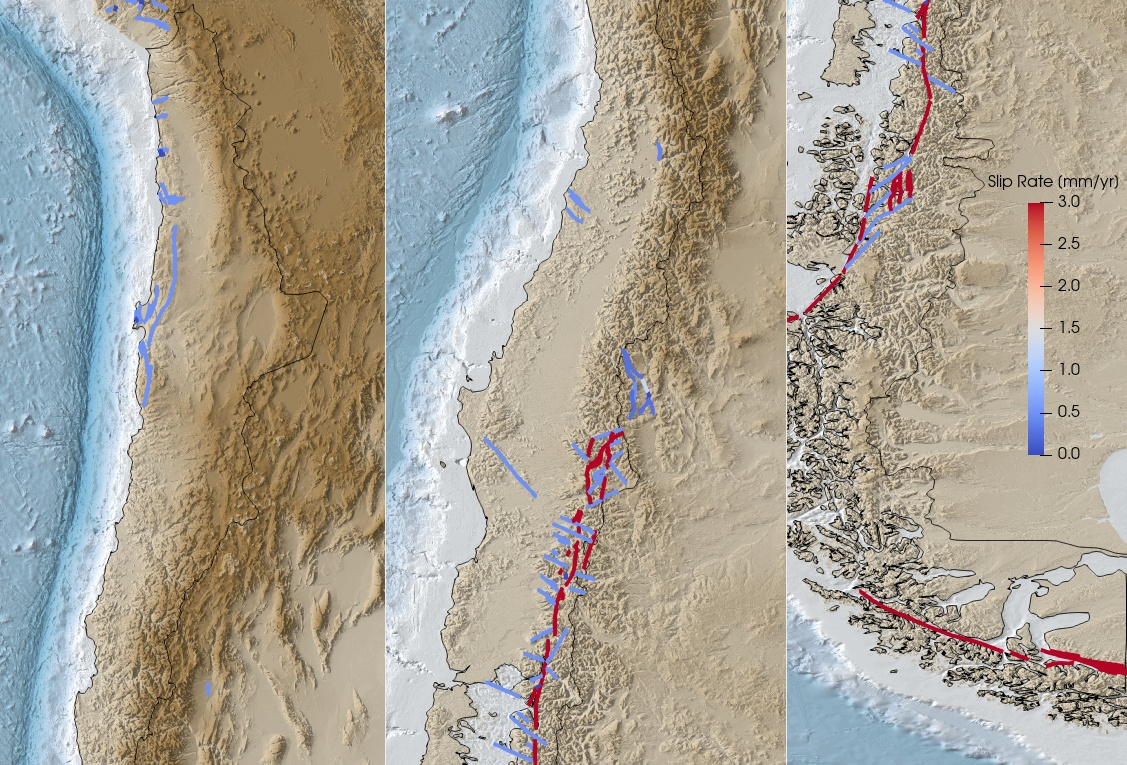
\includegraphics[width=0.6\textwidth]{../figures/slip_rate}
	\end{figure}


\end{frame}

\begin{frame}[t]
	\frametitle{Fault Data}

	Used moment balance $\dot{M}_{\mathrm{long-term}} = \dot{M}_{seismic}$ and fitted a Truncated GR, with $b-$value from regional catalog
	\begin{figure}
		\vspace{0.3cm}
		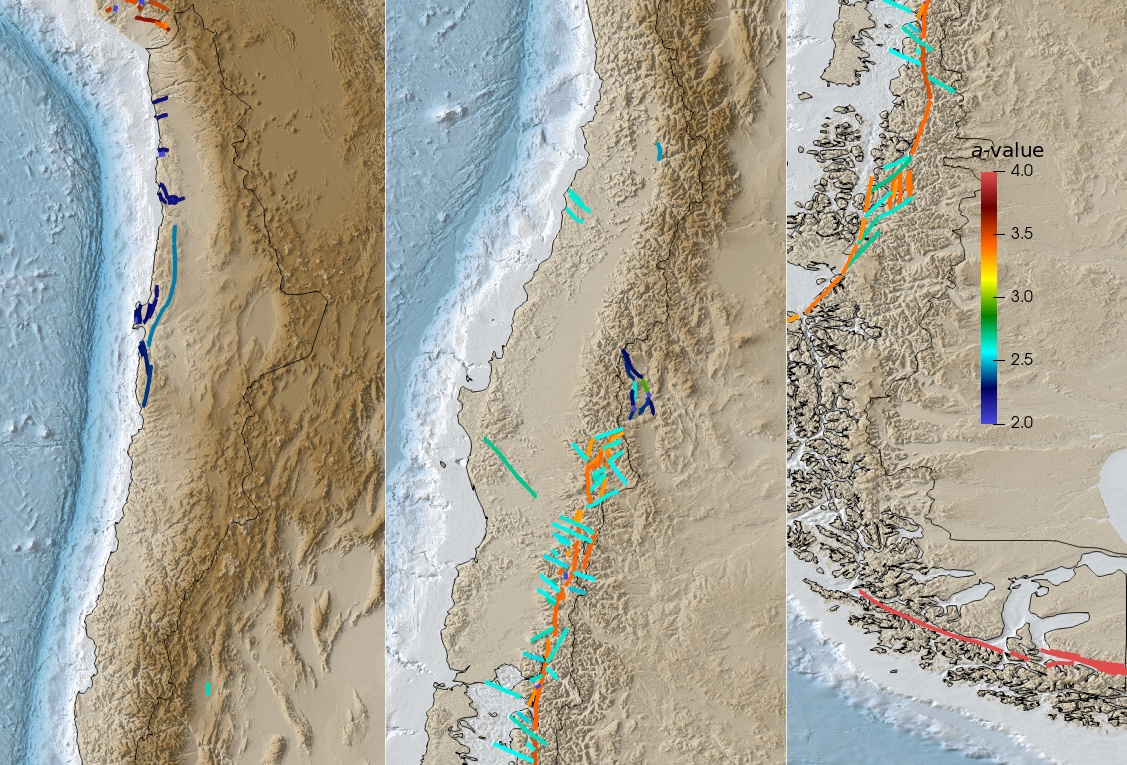
\includegraphics[width=0.6\textwidth]{../figures/a_val_faults}
	\end{figure}
\end{frame}

\begin{frame}[t]
	\frametitle{Ground Motion Models}
	\textbf{Subduction}
	\begin{itemize}
		\item AbrahamsonGulerce2020SInter
		\item ParkerEtAl2020SInter
		\item KuehnEtAl2020SInter
	\end{itemize}
	\textbf{Intra-Slab}
	\begin{itemize}
		\item AbrahamsonGulerce2020SSlab
		\item ParkerEtAl2020SSlab
	\end{itemize}
		\textbf{Crustal}
	\begin{itemize}
		\item AbrahamsonEtAl2014
		\item BooreEtAl2014
		\item CampbellBozorgnia2014
		\item ChiouYoungs2014
	\end{itemize}
\end{frame}

\begin{frame}[t]
	\frametitle{Baseline Hazard Without Faults}

	Displaying PGA at 10\% probability of exceedance in 50 years ($T_r = 475$ years )
	\begin{figure}
		\vspace{0.3cm}
		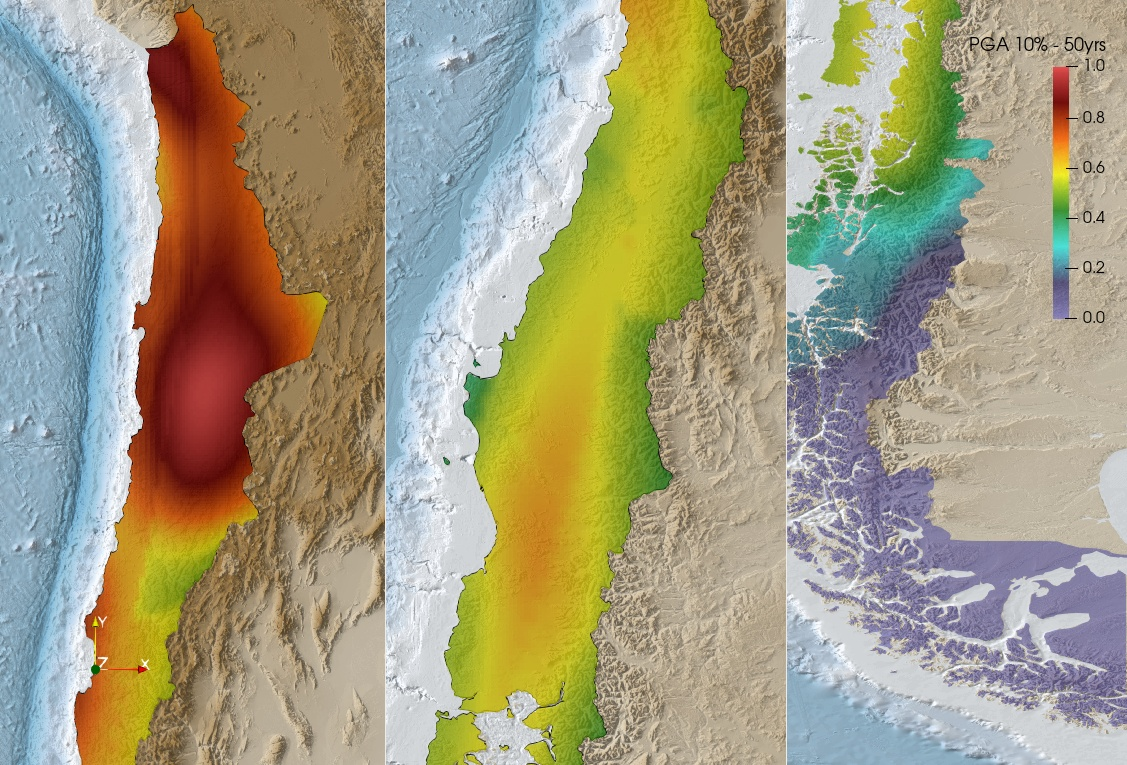
\includegraphics[width=0.6\textwidth]{../figures/nofault_model}
	\end{figure}
\end{frame}

\begin{frame}[t]
	\frametitle{Baseline Hazard With Faults}

	Displaying PGA at 10\% probability of exceedance in 50 years ($T_r = 475$ years )
	\begin{figure}
		\vspace{0.3cm}
		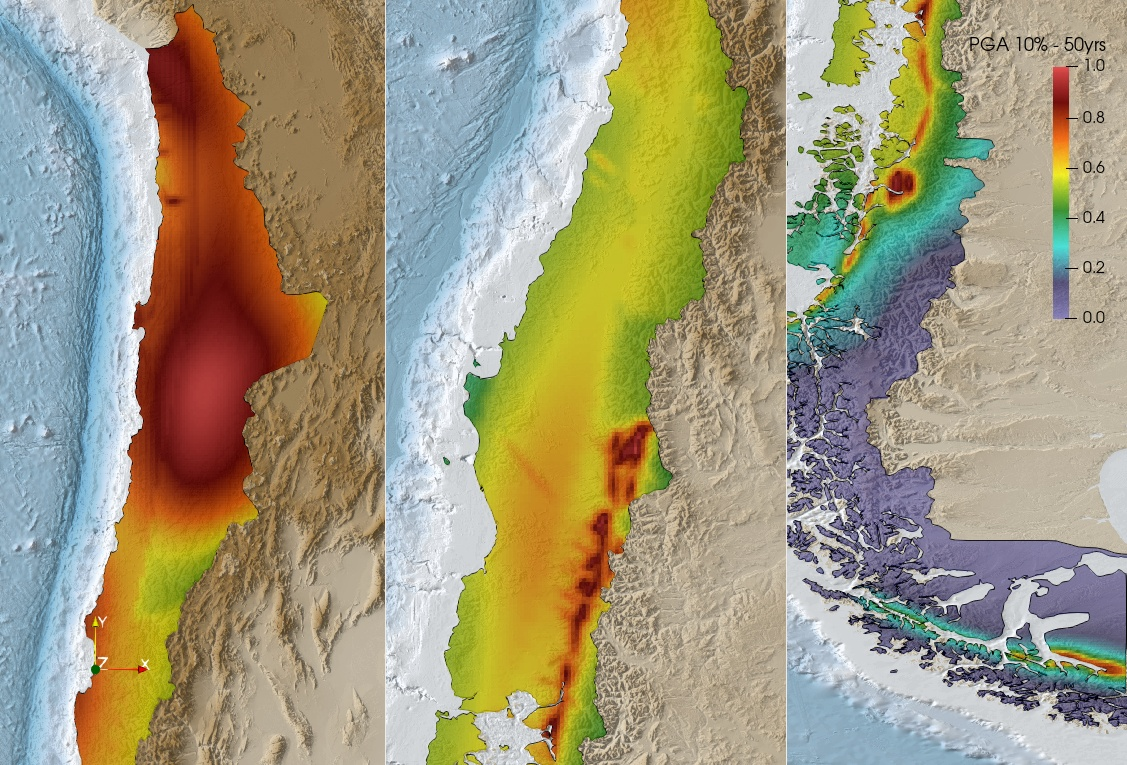
\includegraphics[width=0.6\textwidth]{../figures/fault_model}
	\end{figure}
\end{frame}

\begin{frame}[t]
	\frametitle{Model Comparison - Hazard Curves}

		\begin{columns}
		\column{.6\textwidth}
			\begin{figure}
		\vspace{0.3cm}
		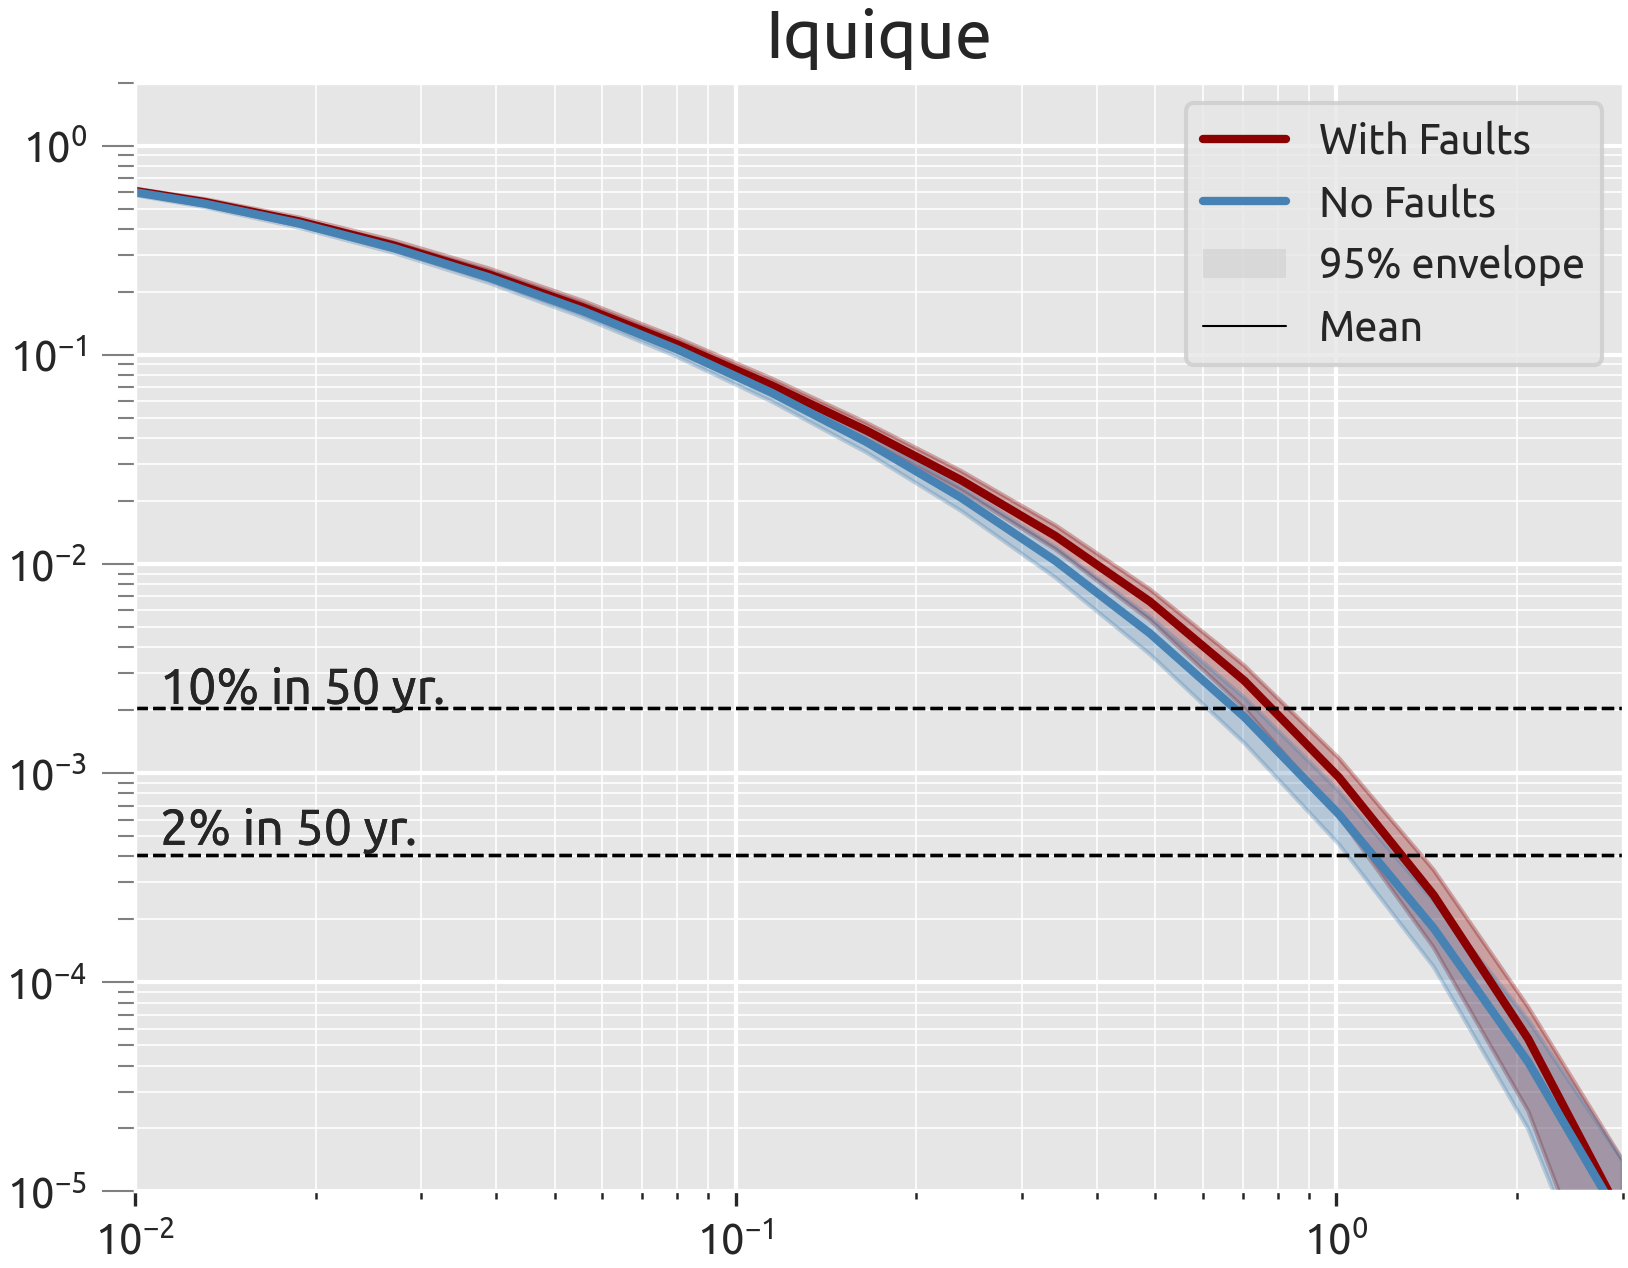
\includegraphics[width=0.8\textwidth]{../figures/Iquique}
	\end{figure}
		\column{.4\textwidth}

		\end{columns}

\end{frame}
\begin{frame}[t]
	\frametitle{Model Comparison - Hazard Curves}

		\begin{columns}
		\column{.6\textwidth}
			\begin{figure}
		\vspace{0.3cm}
		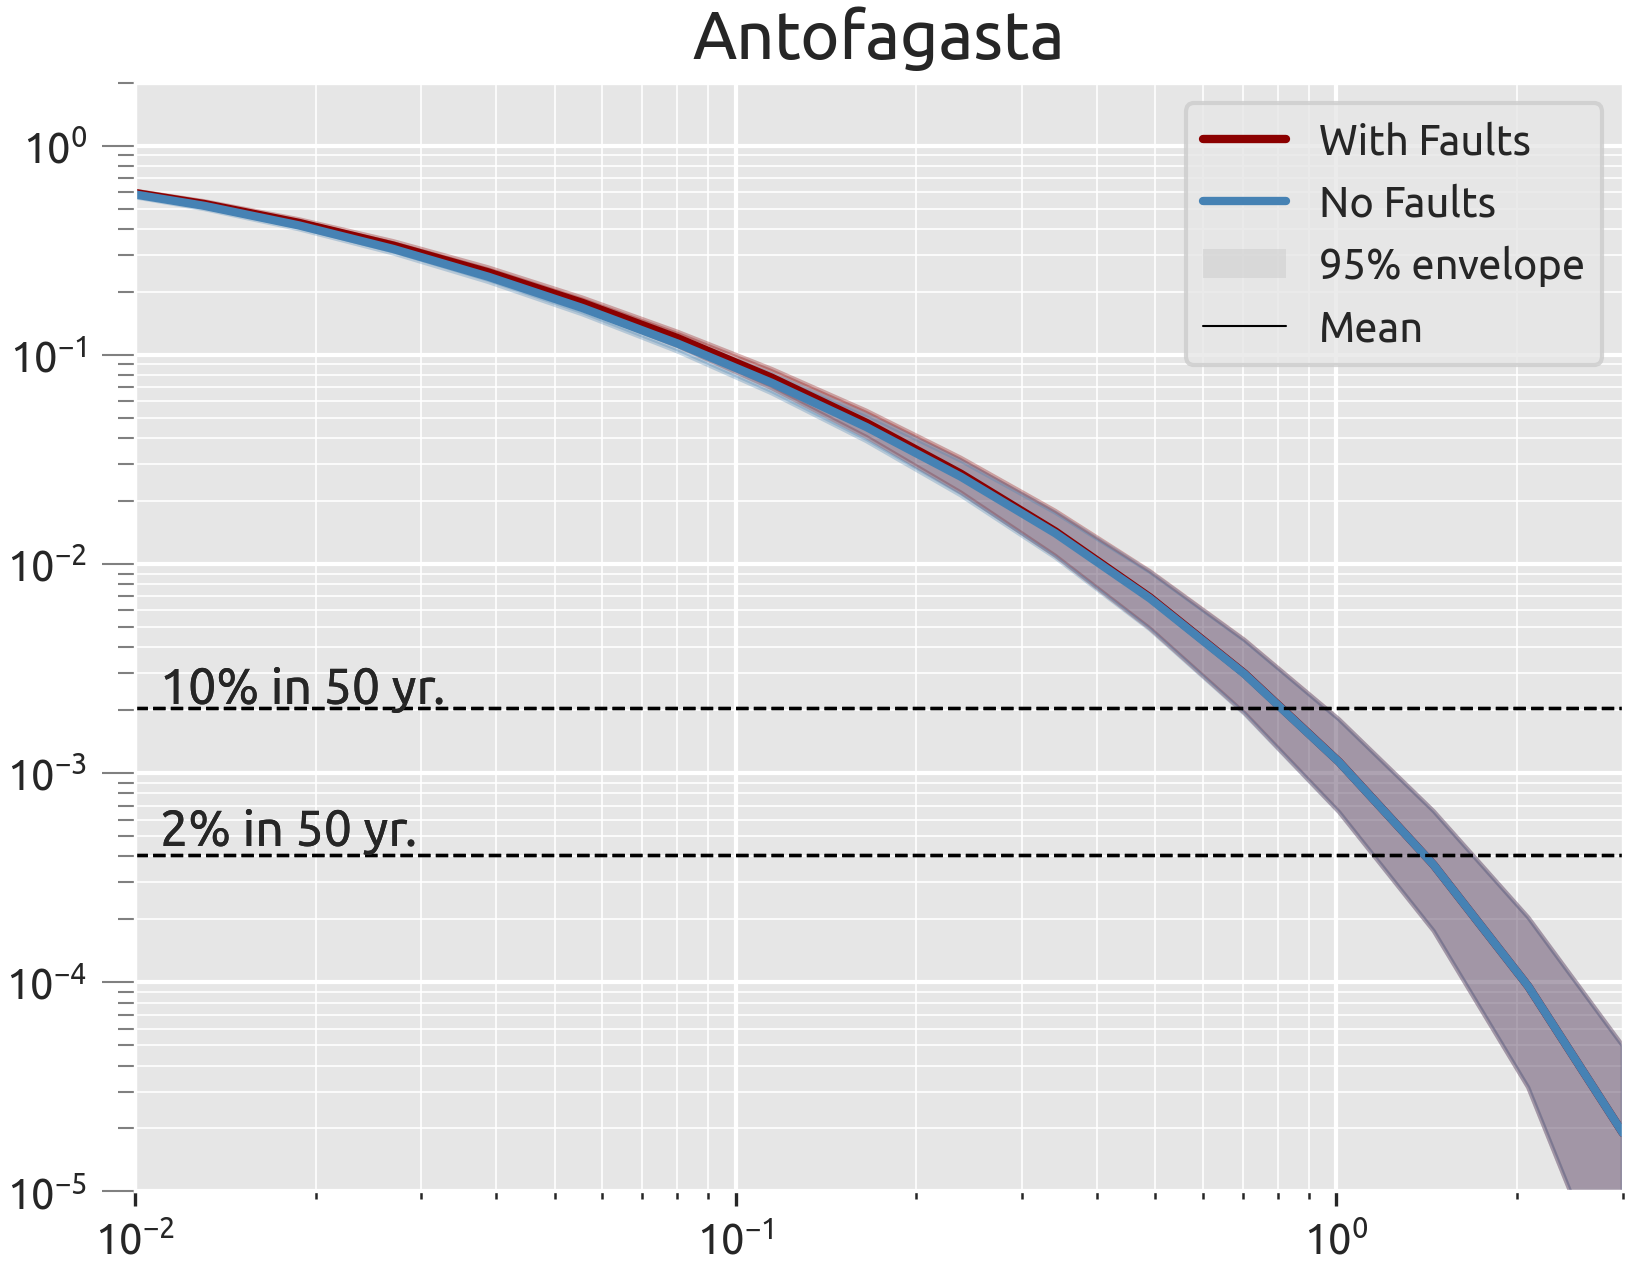
\includegraphics[width=0.8\textwidth]{../figures/Antofagasta}
	\end{figure}
		\column{.4\textwidth}
		\vspace{-1cm}
			\begin{figure}
		\vspace{0.3cm}
		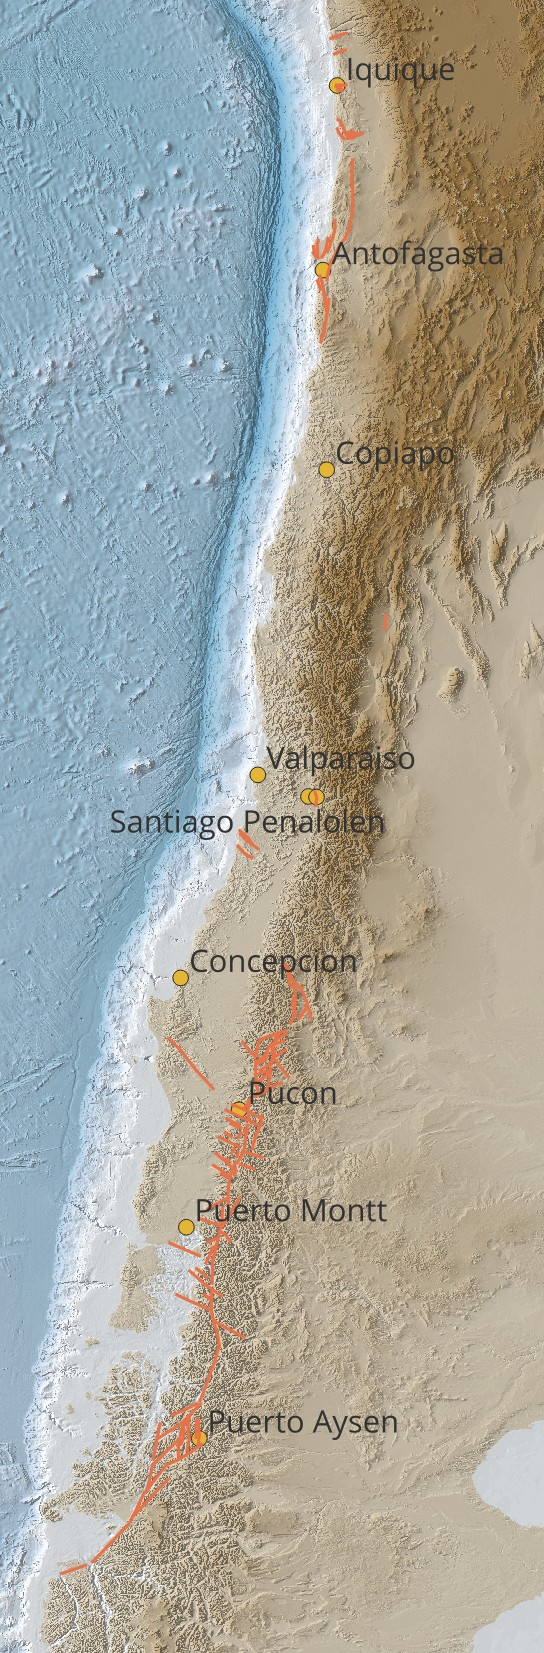
\includegraphics[width=0.4\textwidth]{../figures/cities}
	\end{figure}
		\end{columns}

\end{frame}
	\begin{frame}[t]
	\frametitle{Model Comparison - Hazard Curves}

		\begin{columns}
		\column{.6\textwidth}
			\begin{figure}
		\vspace{0.3cm}
		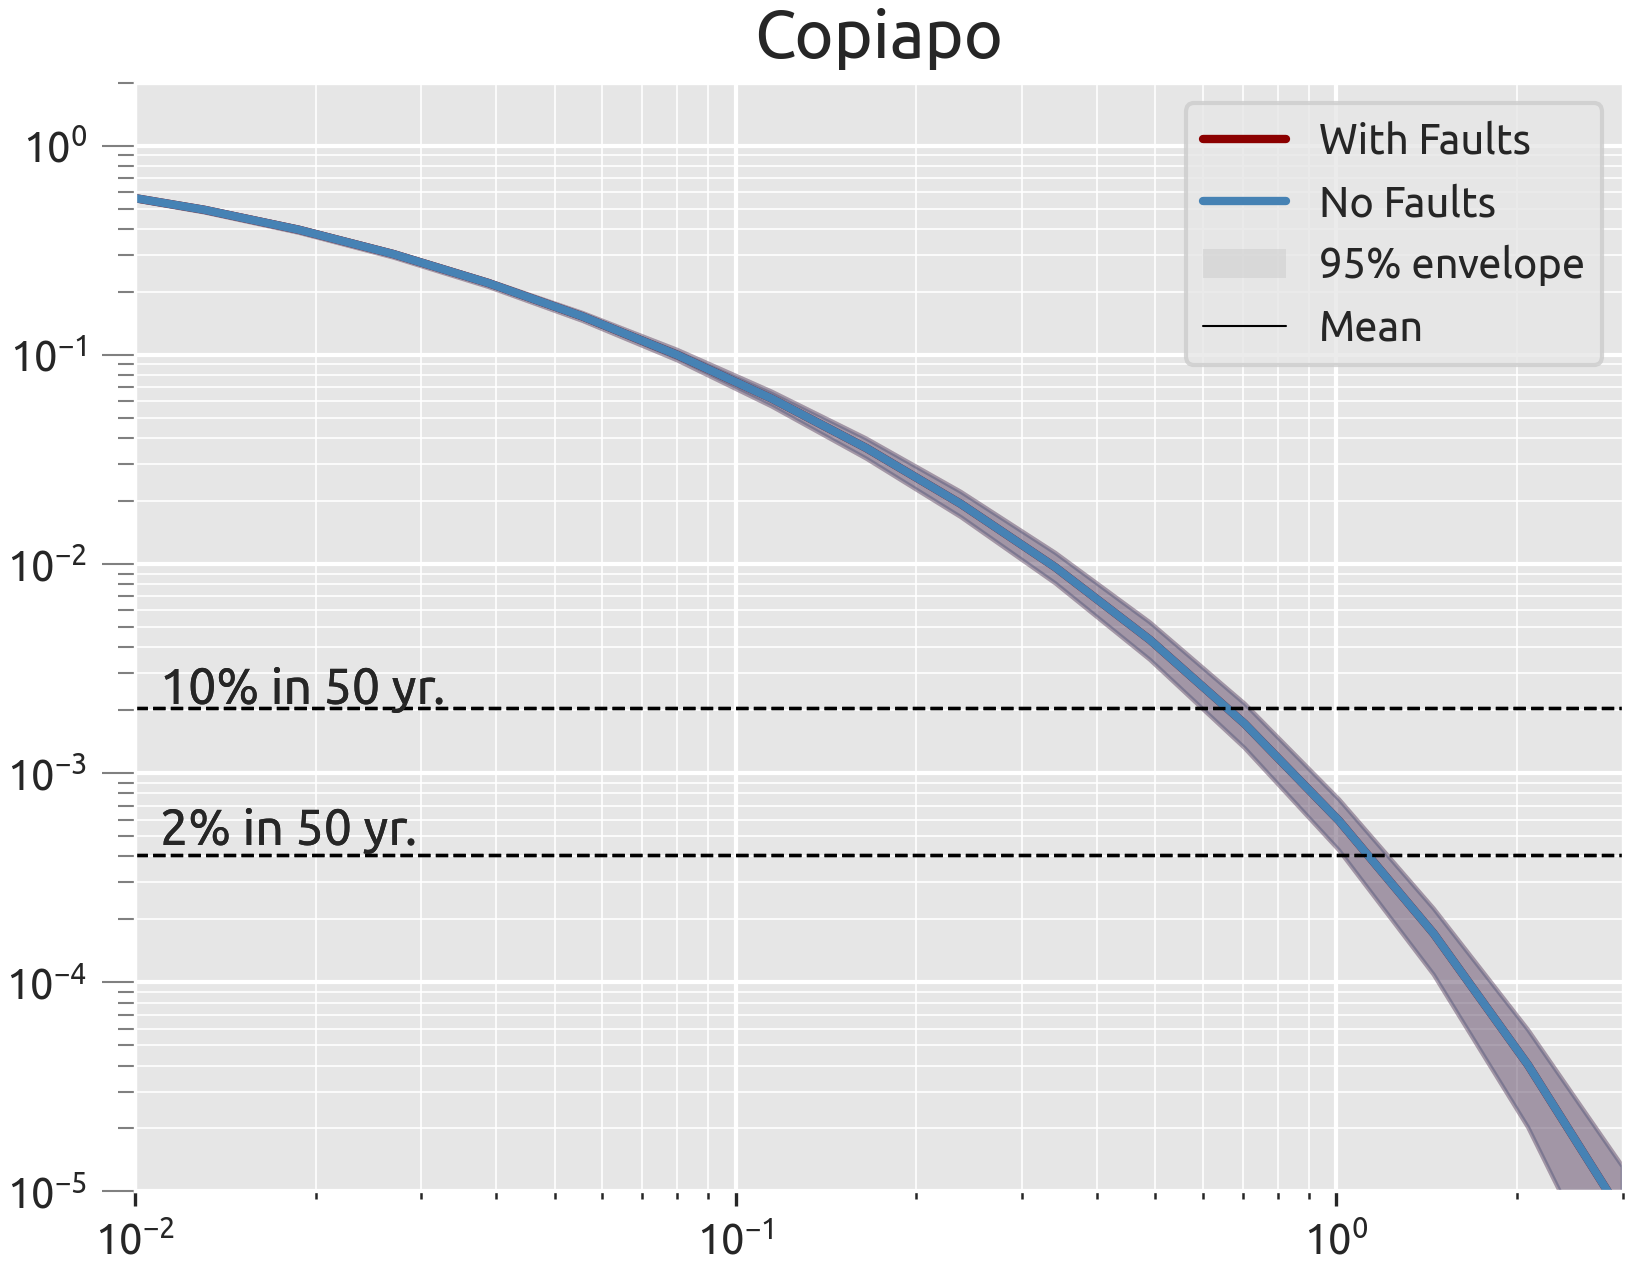
\includegraphics[width=0.8\textwidth]{../figures/Copiapo}
	\end{figure}
		\column{.4\textwidth}
		\vspace{-1cm}
			\begin{figure}
		\vspace{0.3cm}
		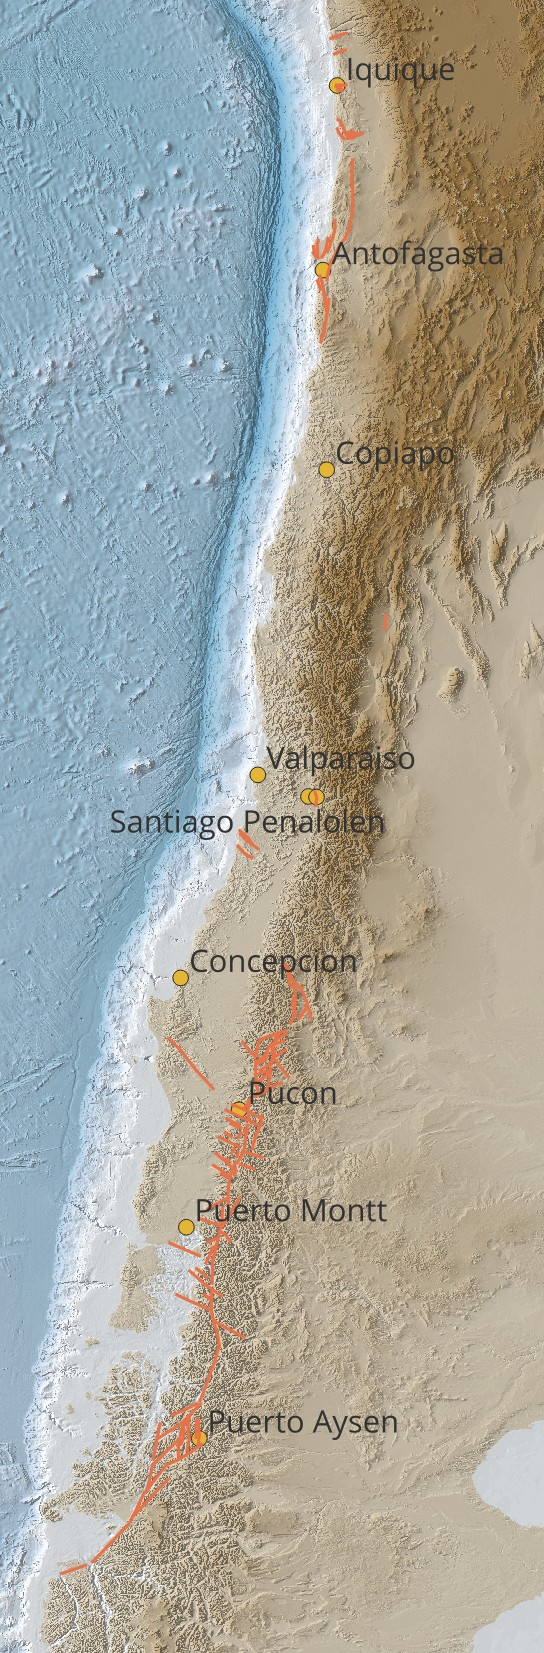
\includegraphics[width=0.4\textwidth]{../figures/cities}
	\end{figure}
		\end{columns}

\end{frame}
	\begin{frame}[t]
	\frametitle{Model Comparison - Hazard Curves}

		\begin{columns}
		\column{.6\textwidth}
			\begin{figure}
		\vspace{0.3cm}
		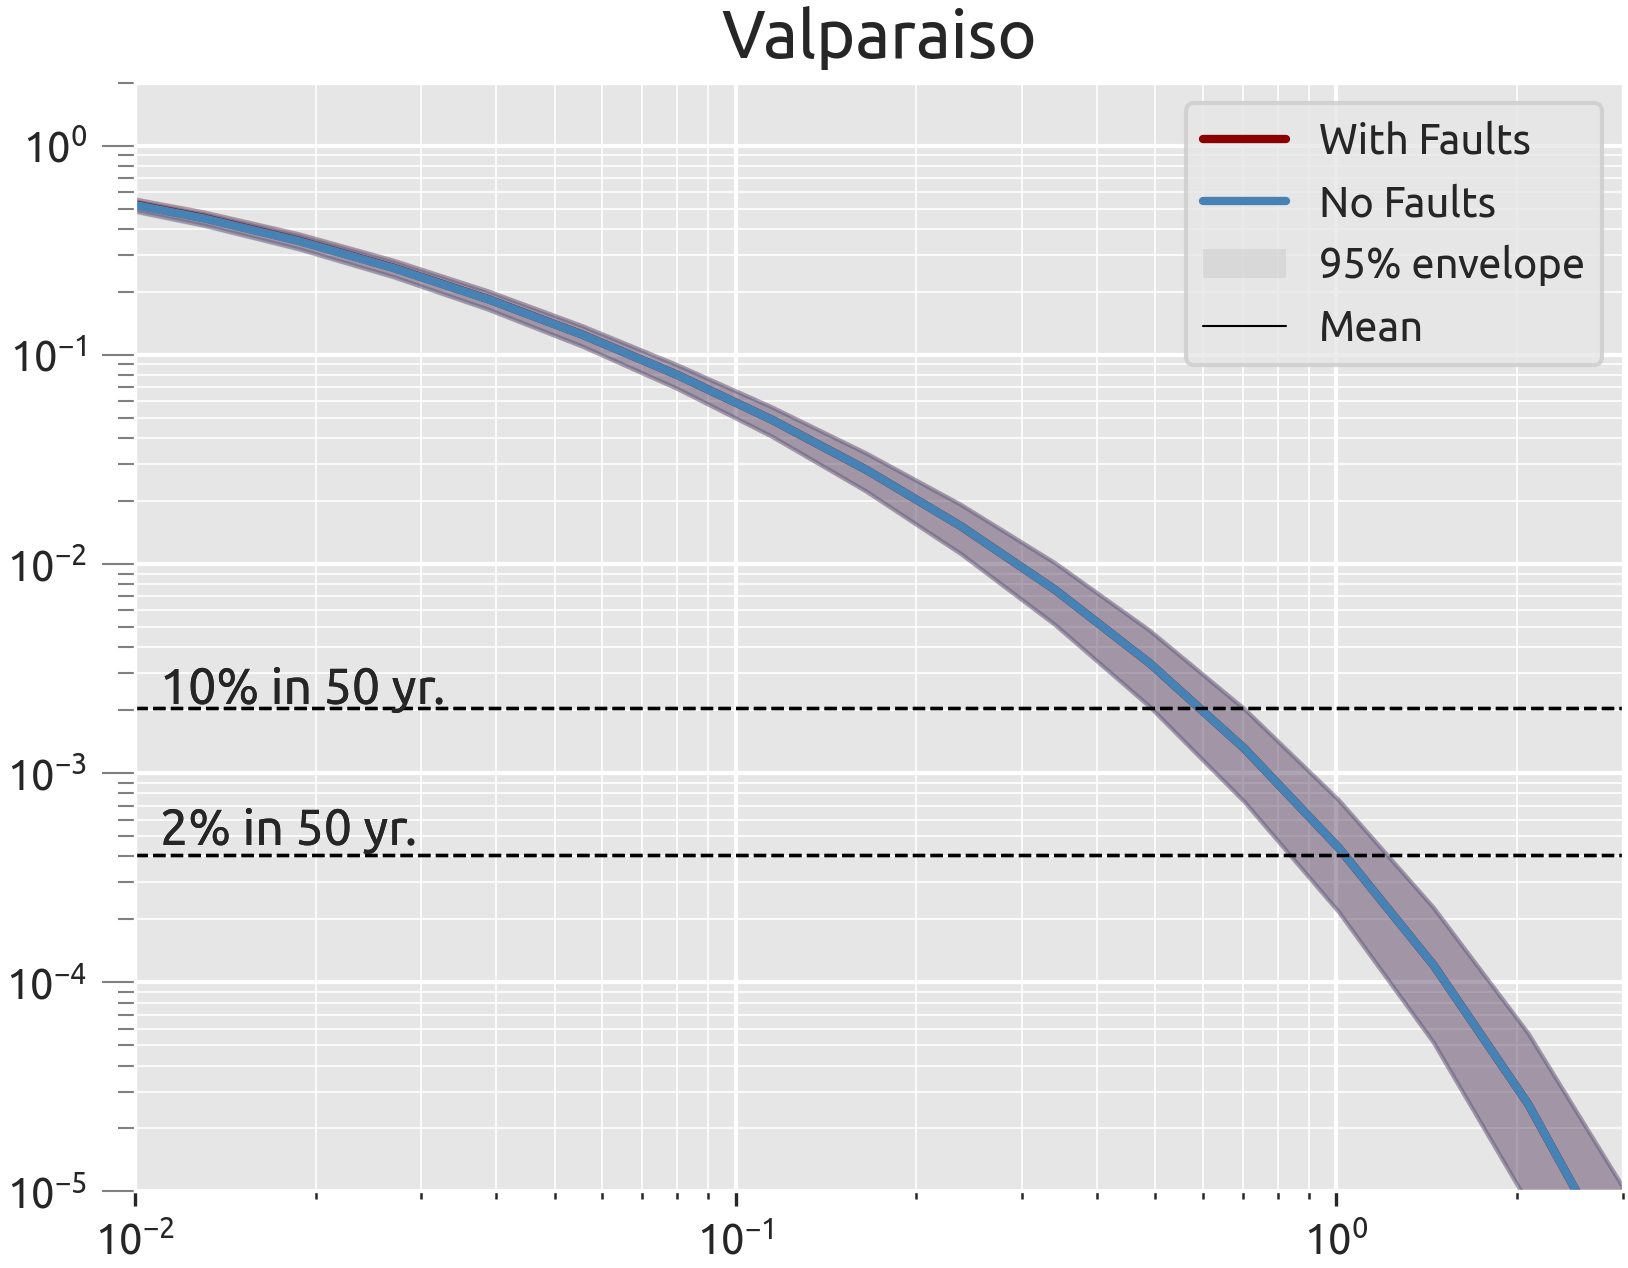
\includegraphics[width=0.8\textwidth]{../figures/Valparaiso}
	\end{figure}
		\column{.4\textwidth}
		\vspace{-1cm}
			\begin{figure}
		\vspace{0.3cm}
		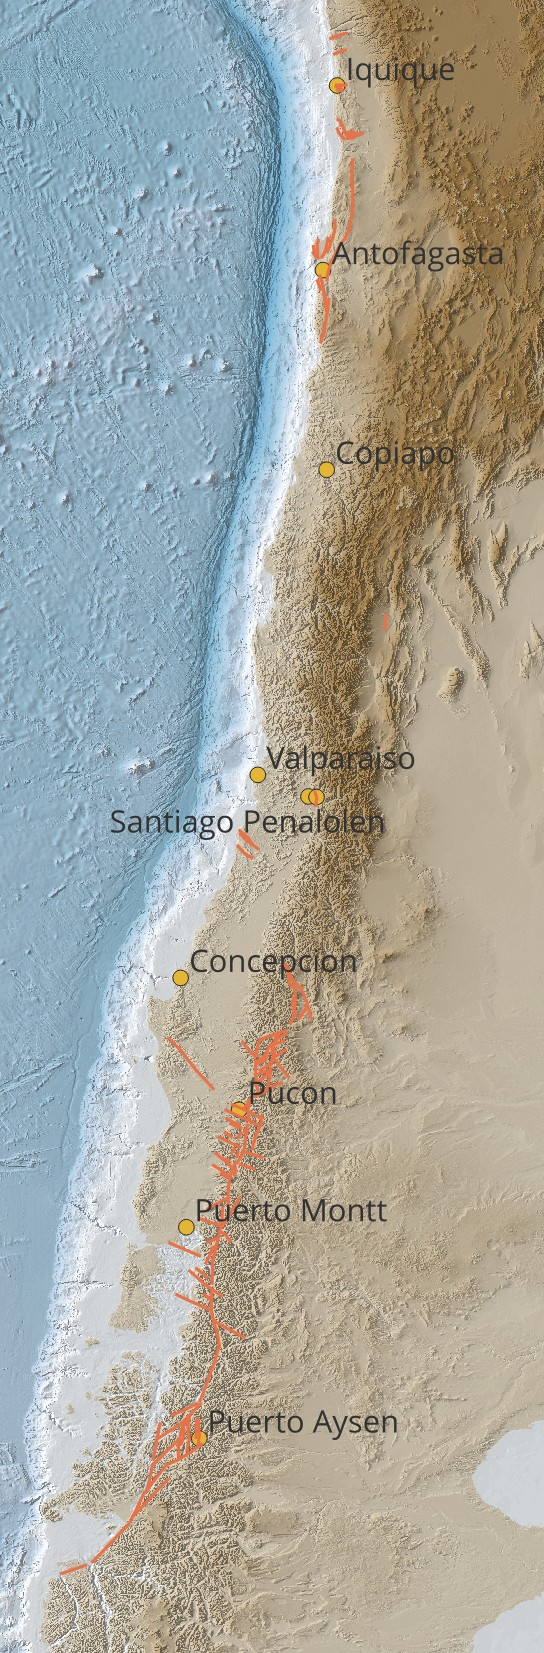
\includegraphics[width=0.4\textwidth]{../figures/cities}
	\end{figure}
		\end{columns}

\end{frame}
	\begin{frame}[t]
	\frametitle{Model Comparison - Hazard Curves}

		\begin{columns}
		\column{.6\textwidth}
			\begin{figure}
		\vspace{0.3cm}
		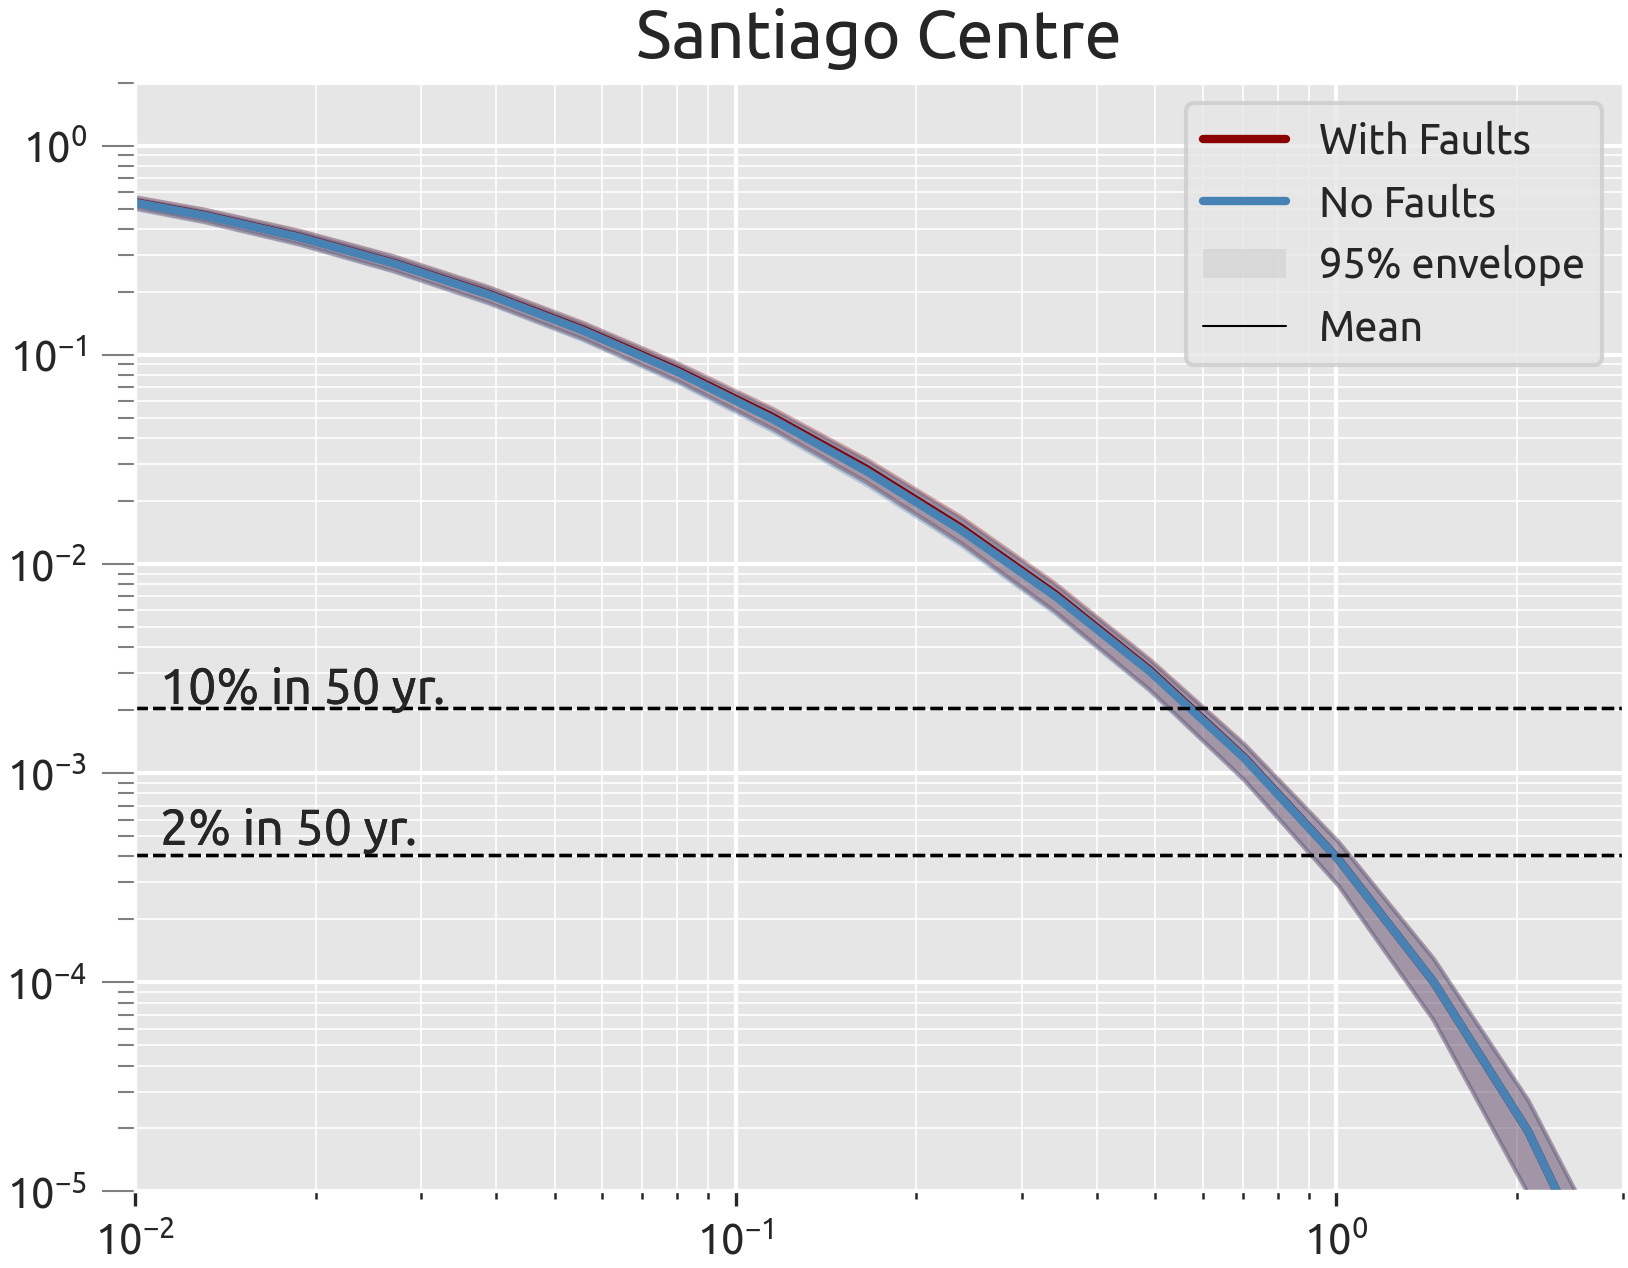
\includegraphics[width=0.8\textwidth]{../figures/Santiago Centre}
	\end{figure}
		\column{.4\textwidth}
		\vspace{-1cm}
			\begin{figure}
		\vspace{0.3cm}
		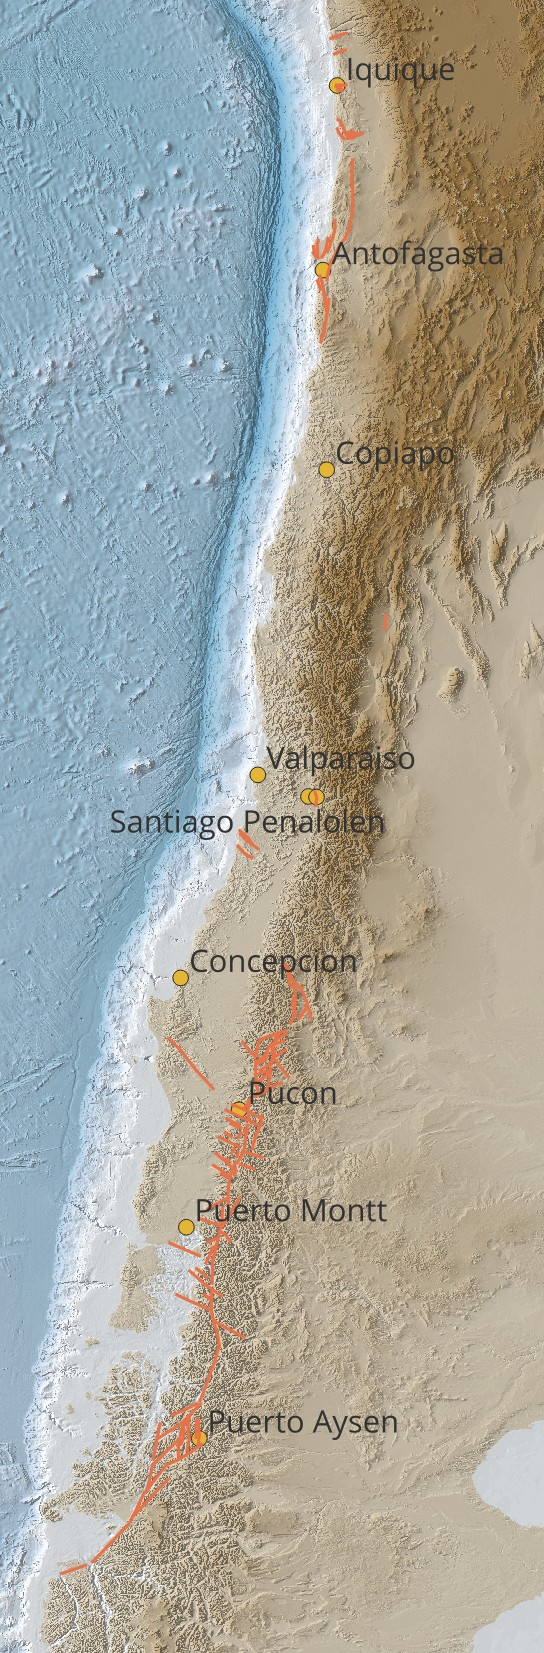
\includegraphics[width=0.4\textwidth]{../figures/cities}
	\end{figure}
		\end{columns}

\end{frame}
	\begin{frame}[t]
	\frametitle{Model Comparison - Hazard Curves}

		\begin{columns}
		\column{.6\textwidth}
			\begin{figure}
		\vspace{0.3cm}
		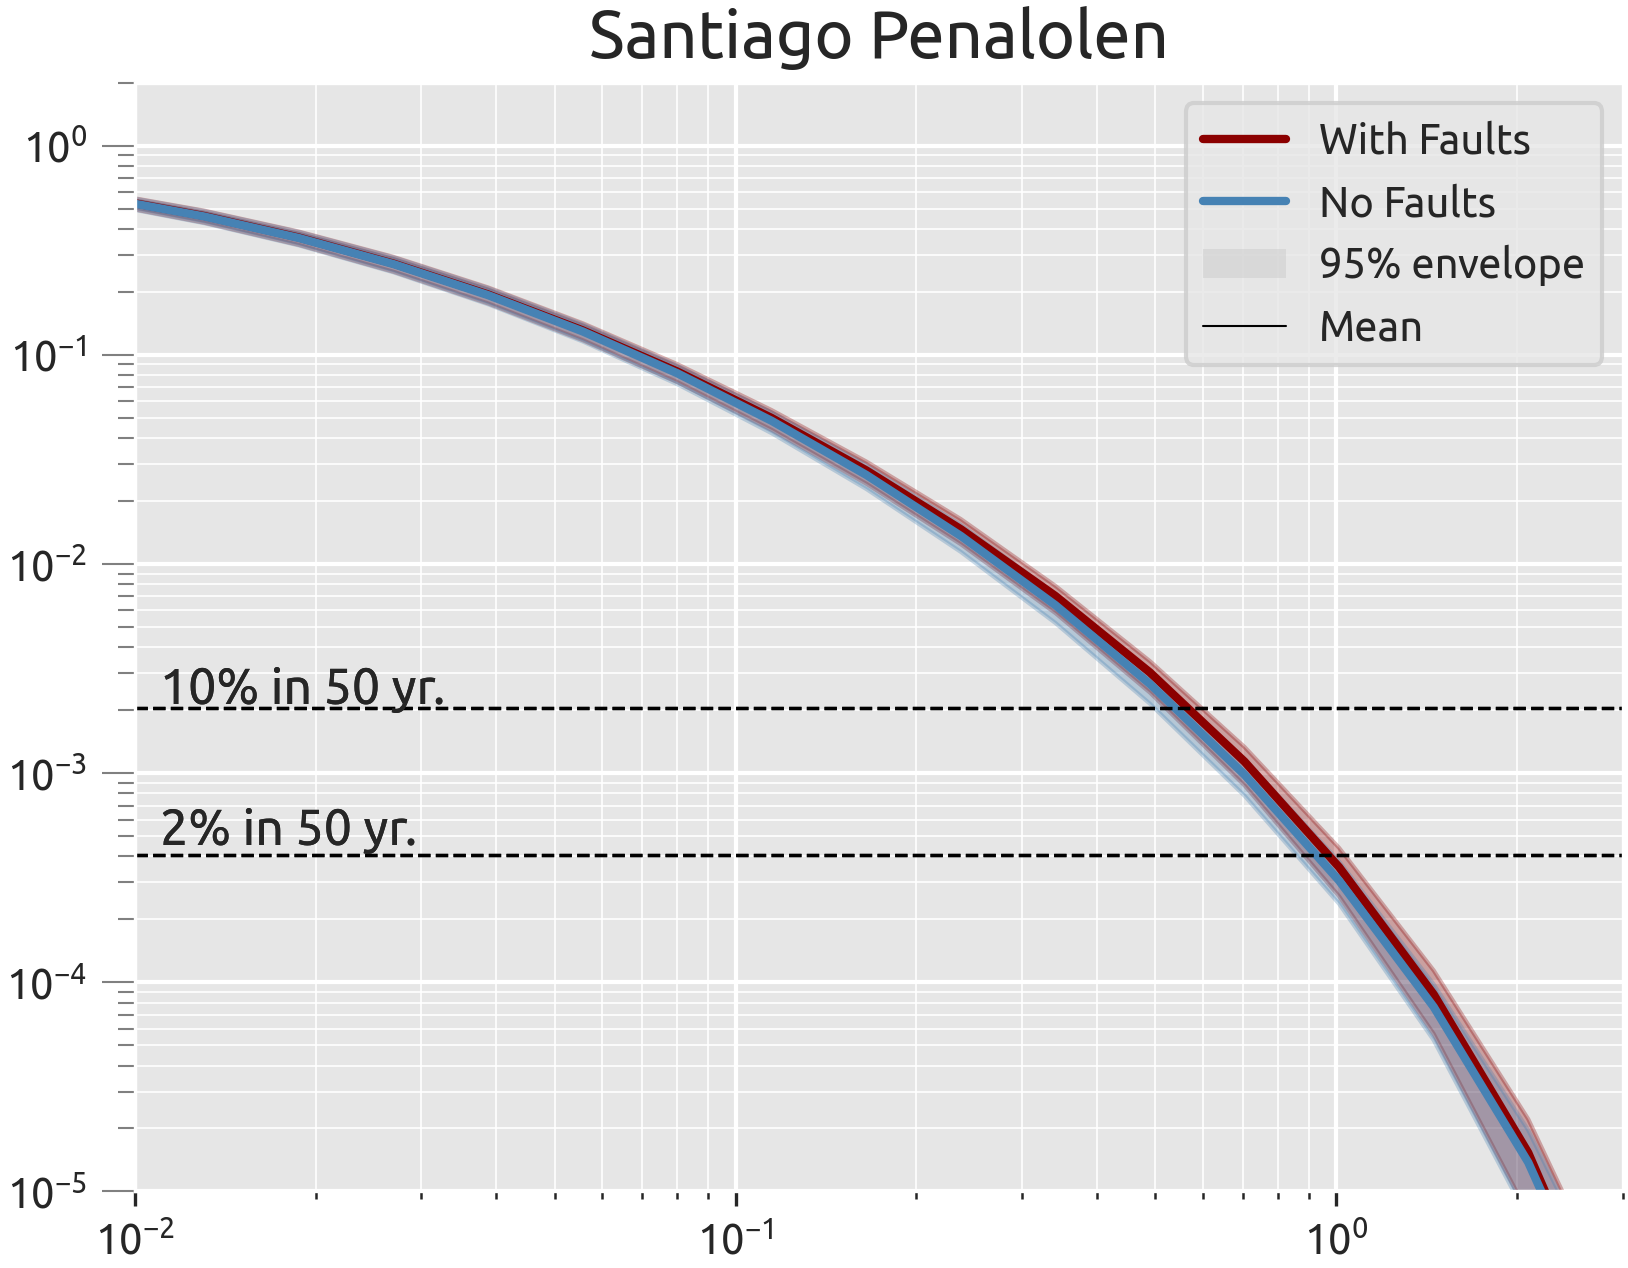
\includegraphics[width=0.8\textwidth]{../figures/Santiago Penalolen}
	\end{figure}
		\column{.4\textwidth}
		\vspace{-1cm}
			\begin{figure}
		\vspace{0.3cm}
		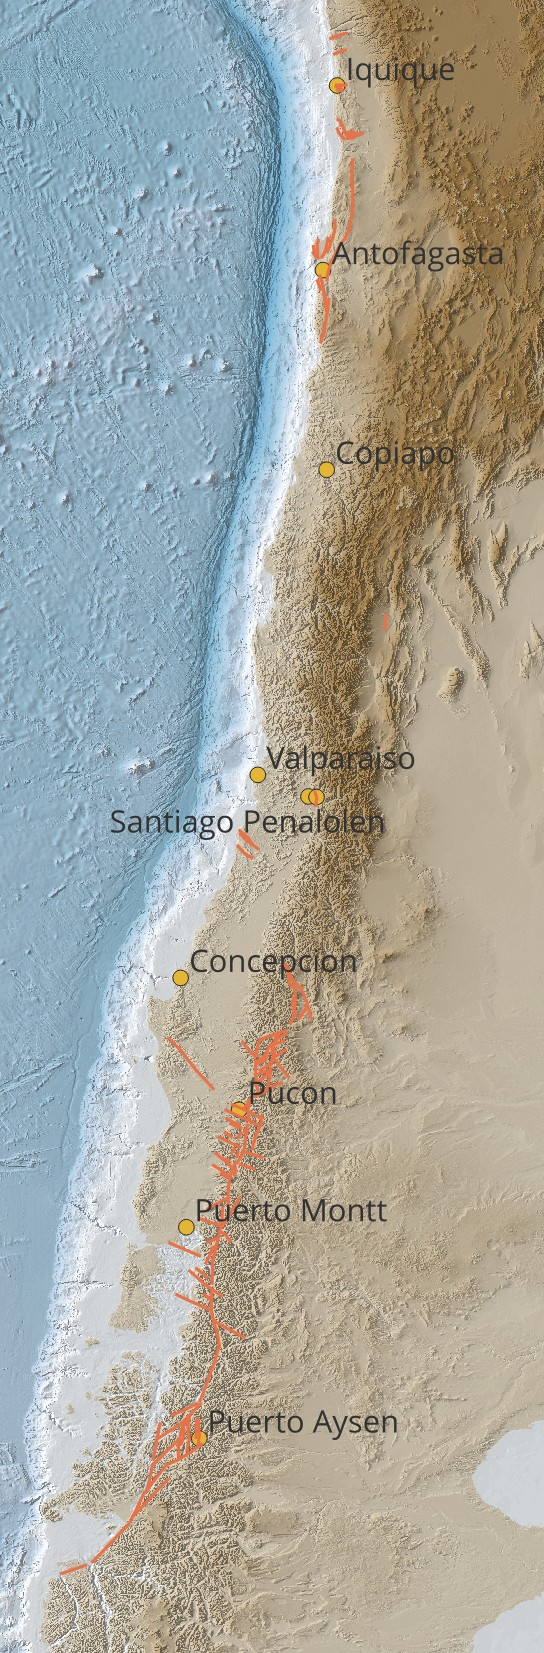
\includegraphics[width=0.4\textwidth]{../figures/cities}
	\end{figure}
		\end{columns}

\end{frame}
	\begin{frame}[t]
	\frametitle{Model Comparison - Hazard Curves}

		\begin{columns}
		\column{.6\textwidth}
			\begin{figure}
		\vspace{0.3cm}
		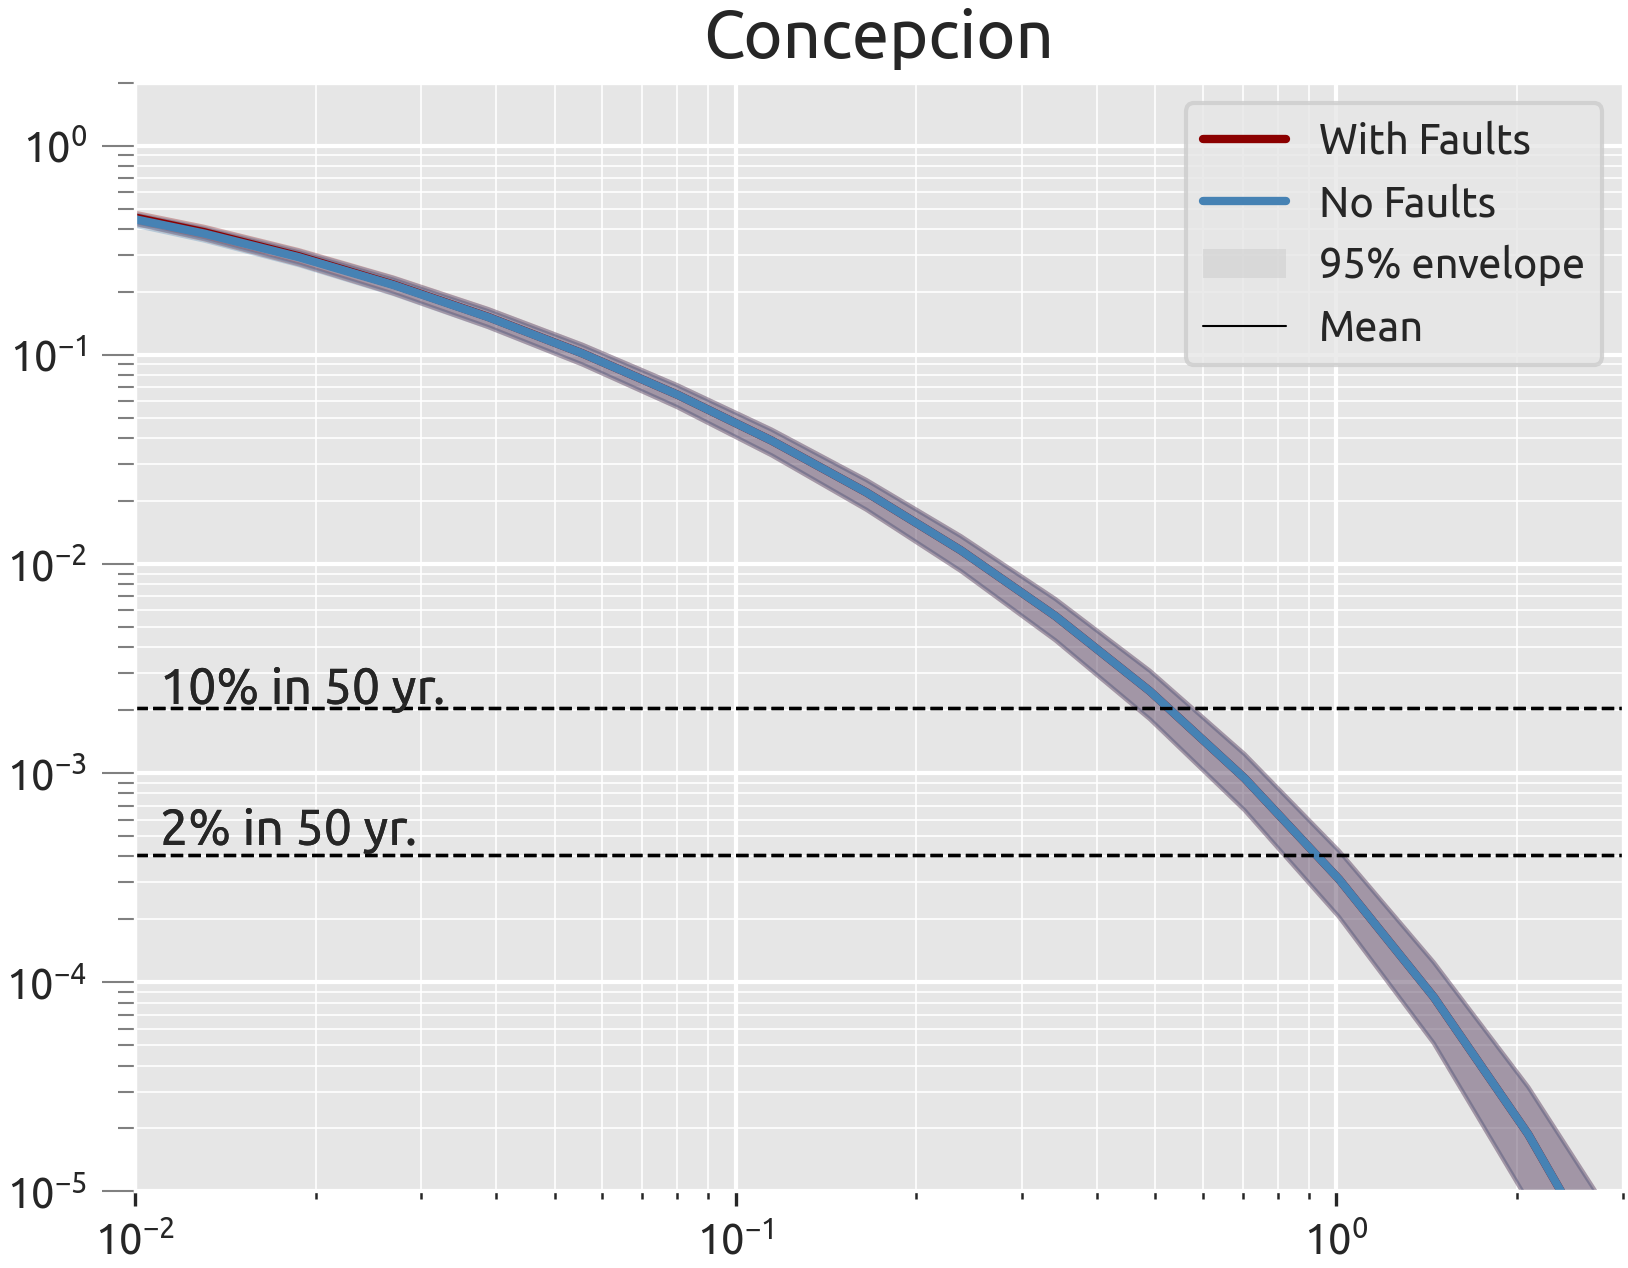
\includegraphics[width=0.8\textwidth]{../figures/Concepcion}
	\end{figure}
		\column{.4\textwidth}
		\vspace{-1cm}
			\begin{figure}
		\vspace{0.3cm}
		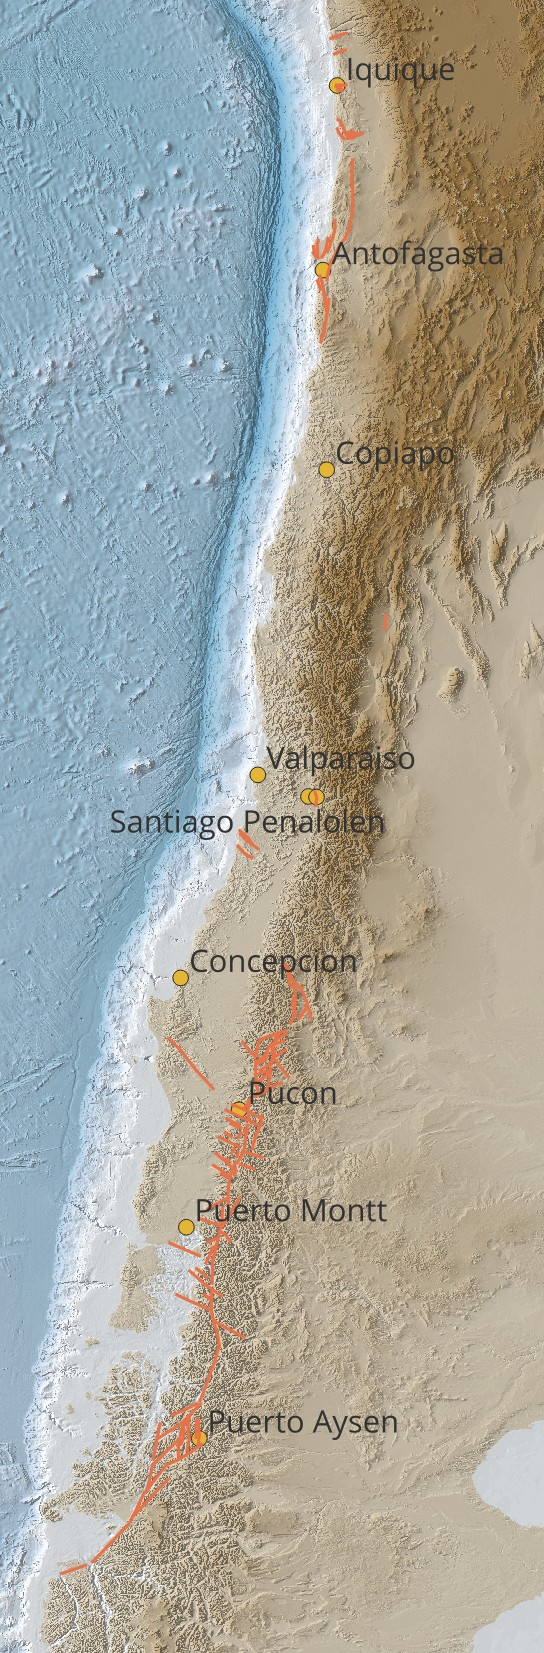
\includegraphics[width=0.4\textwidth]{../figures/cities}
	\end{figure}
		\end{columns}

\end{frame}
	\begin{frame}[t]
	\frametitle{Model Comparison - Hazard Curves}

		\begin{columns}
		\column{.6\textwidth}
			\begin{figure}
		\vspace{0.3cm}
		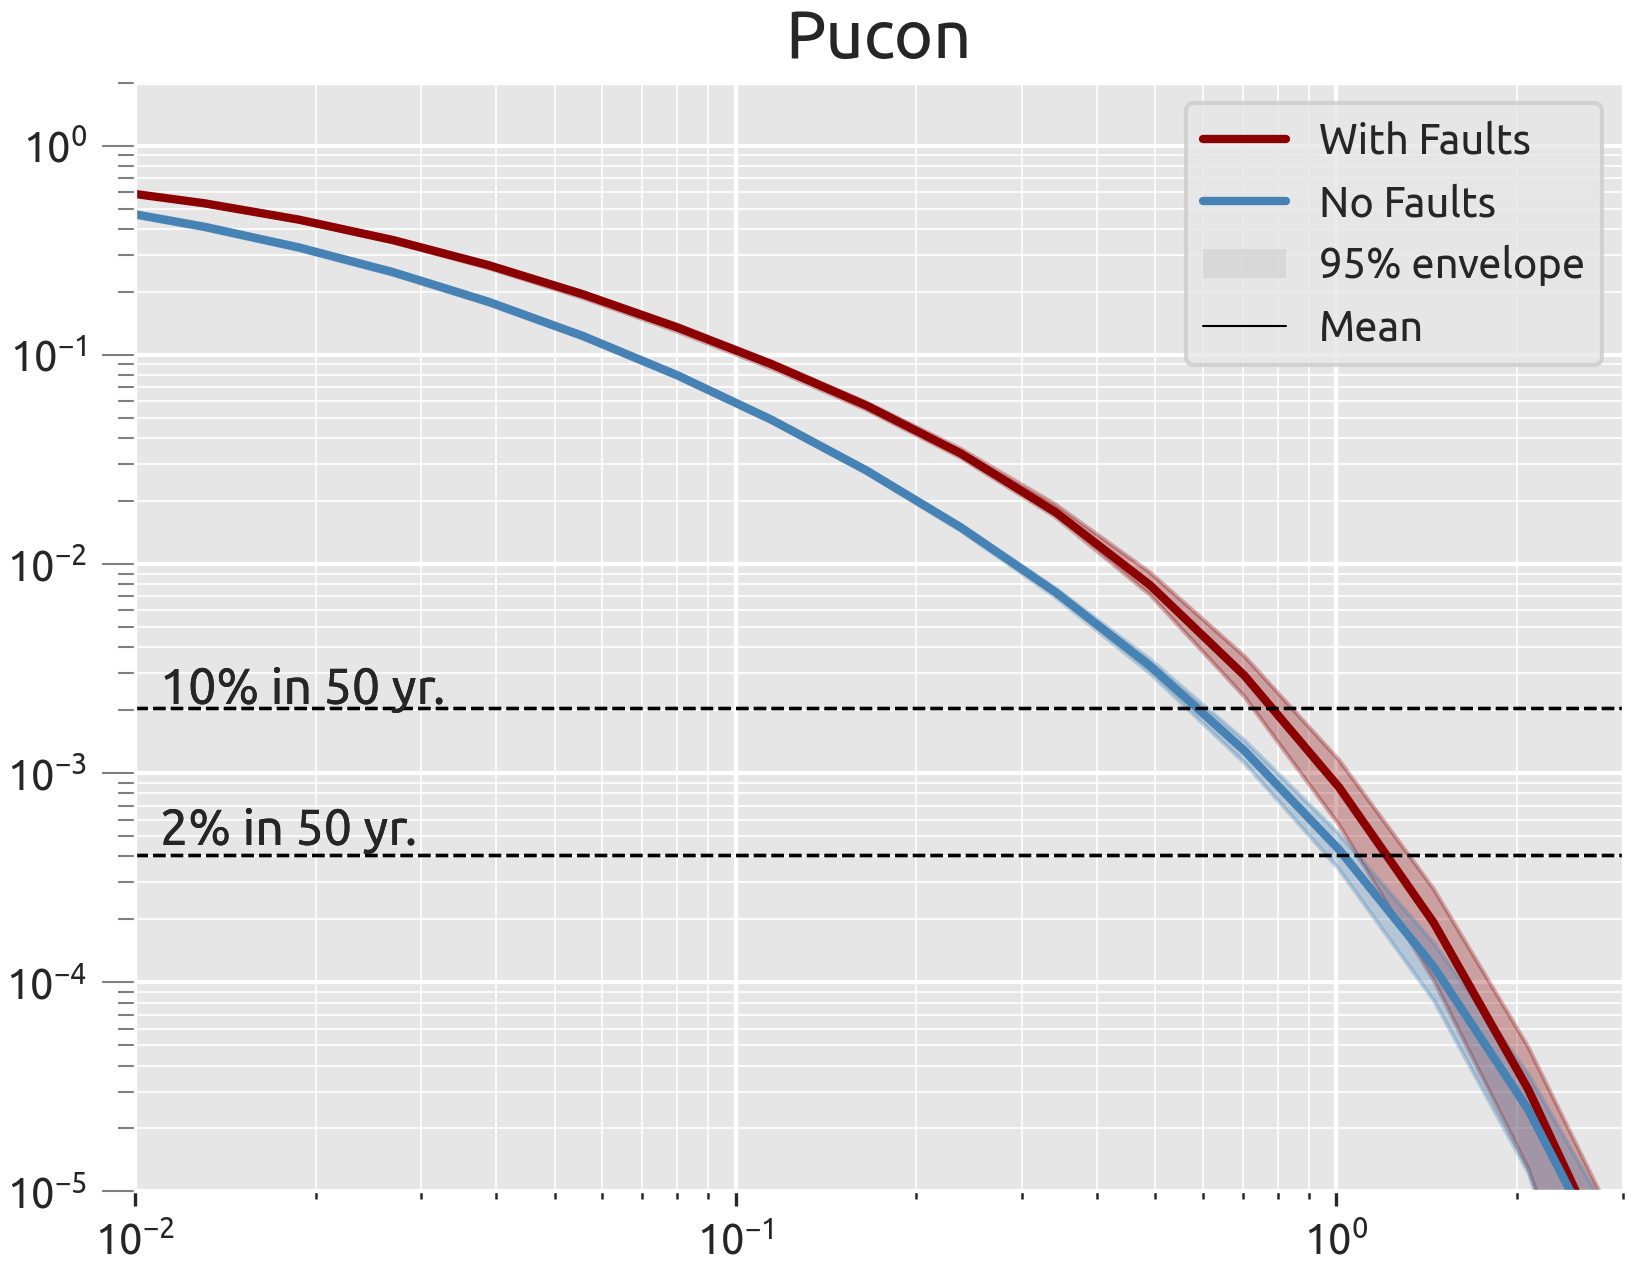
\includegraphics[width=0.8\textwidth]{../figures/Pucon}
	\end{figure}
		\column{.4\textwidth}
		\vspace{-1cm}
			\begin{figure}
		\vspace{0.3cm}
		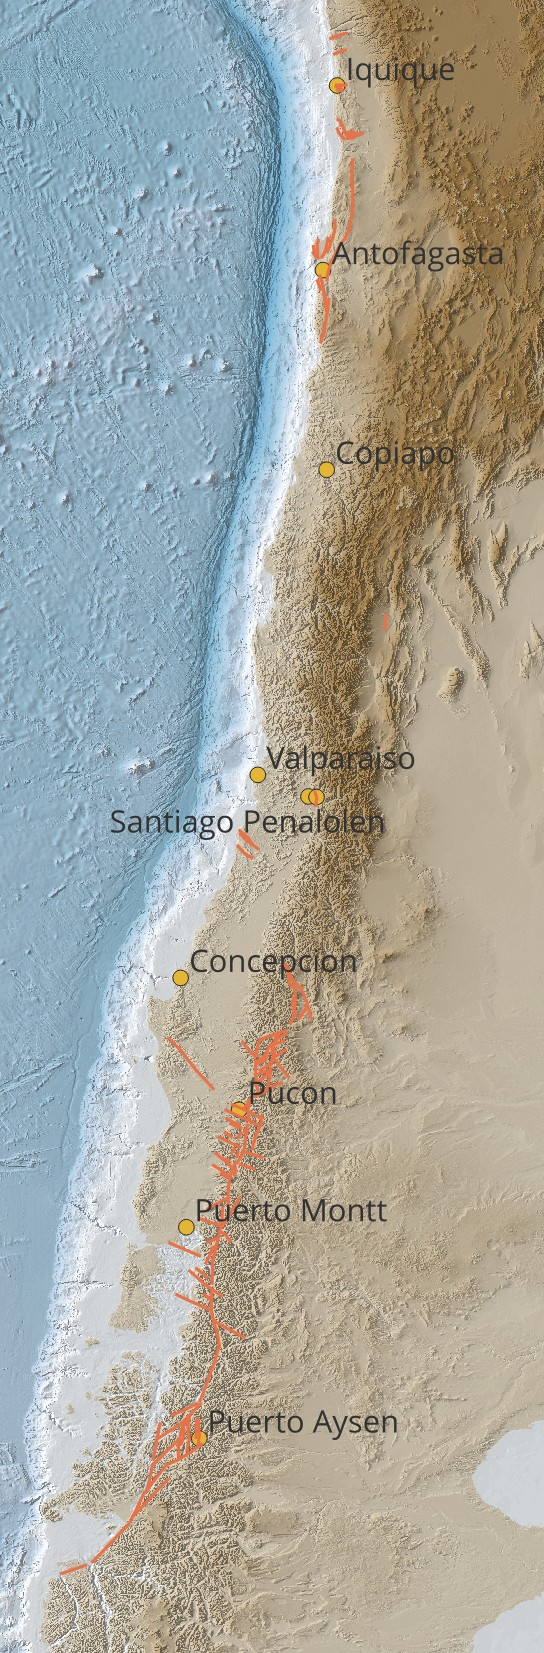
\includegraphics[width=0.4\textwidth]{../figures/cities}
	\end{figure}
		\end{columns}

\end{frame}
	\begin{frame}[t]
	\frametitle{Model Comparison - Hazard Curves}

		\begin{columns}
		\column{.6\textwidth}
			\begin{figure}
		\vspace{0.3cm}
		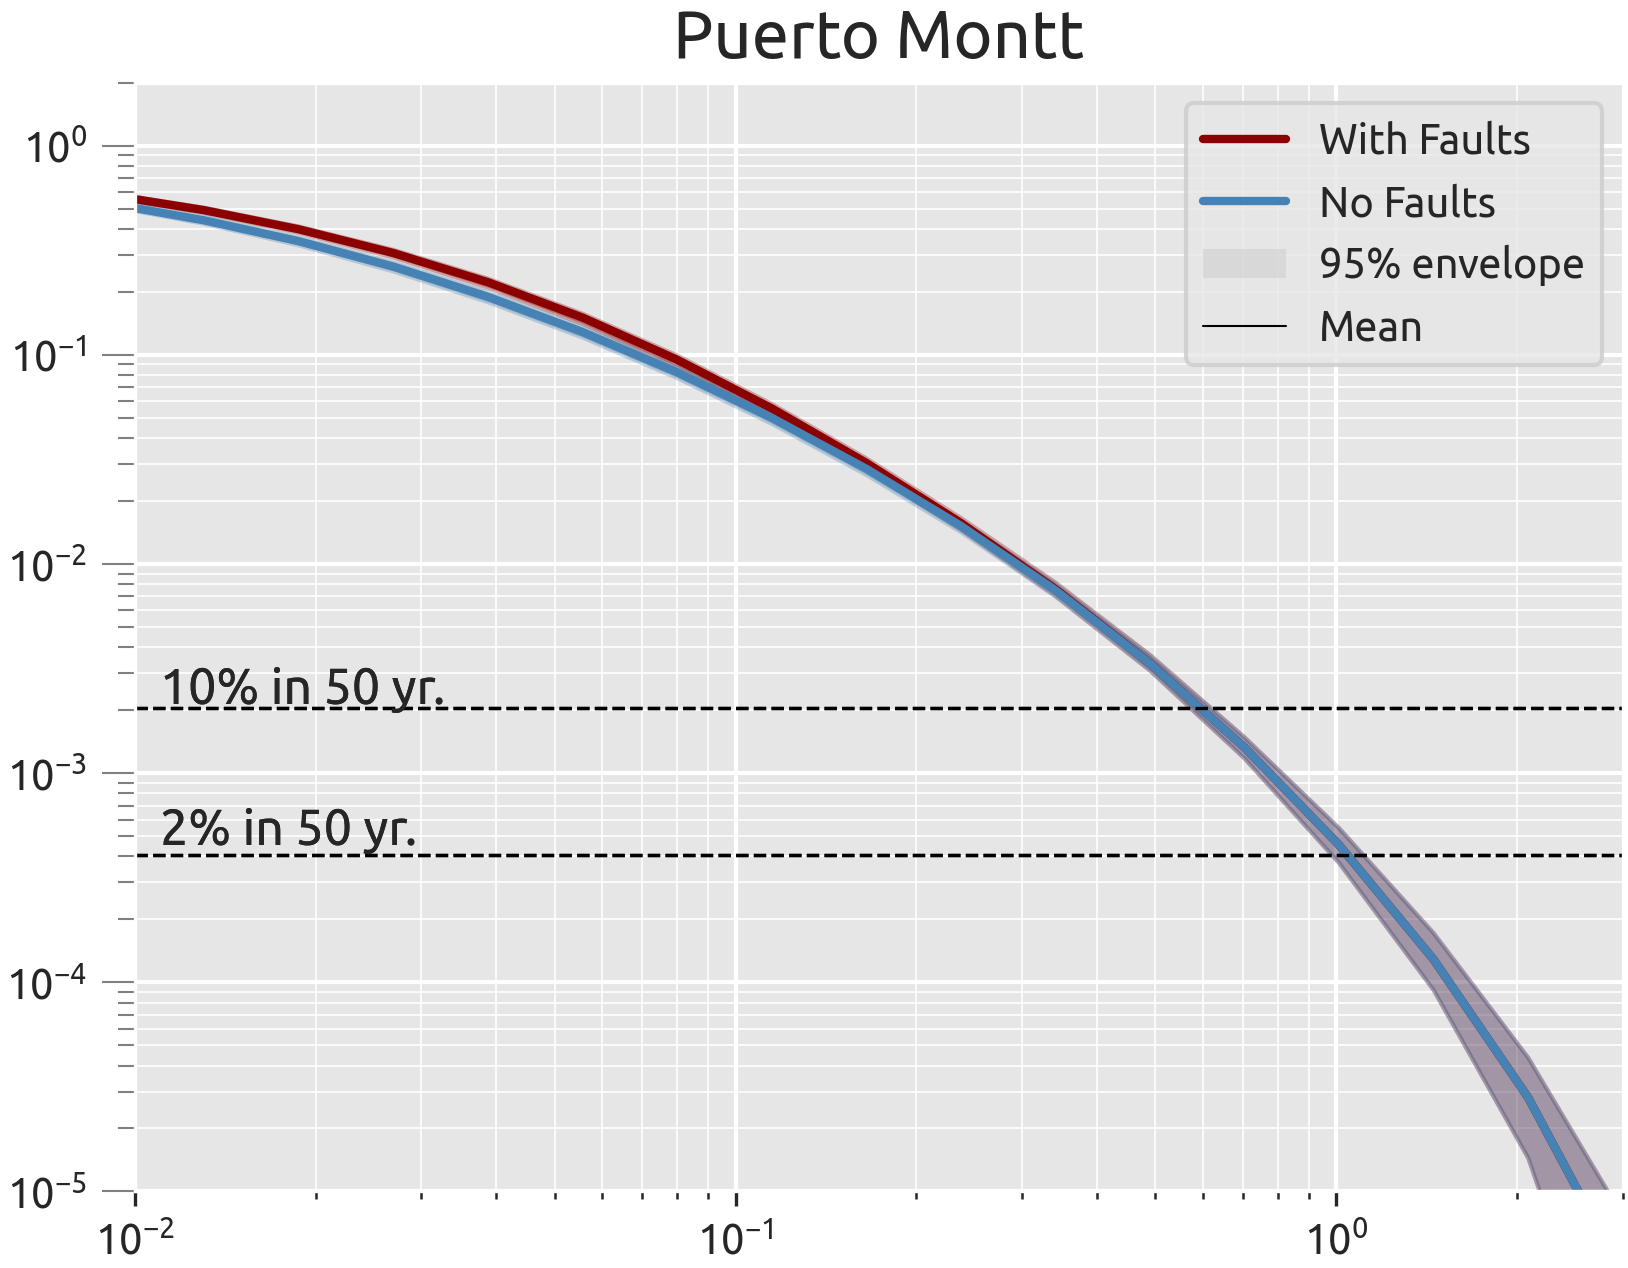
\includegraphics[width=0.8\textwidth]{../figures/Puerto Montt}
	\end{figure}
		\column{.4\textwidth}
		\vspace{-1cm}
			\begin{figure}
		\vspace{0.3cm}
		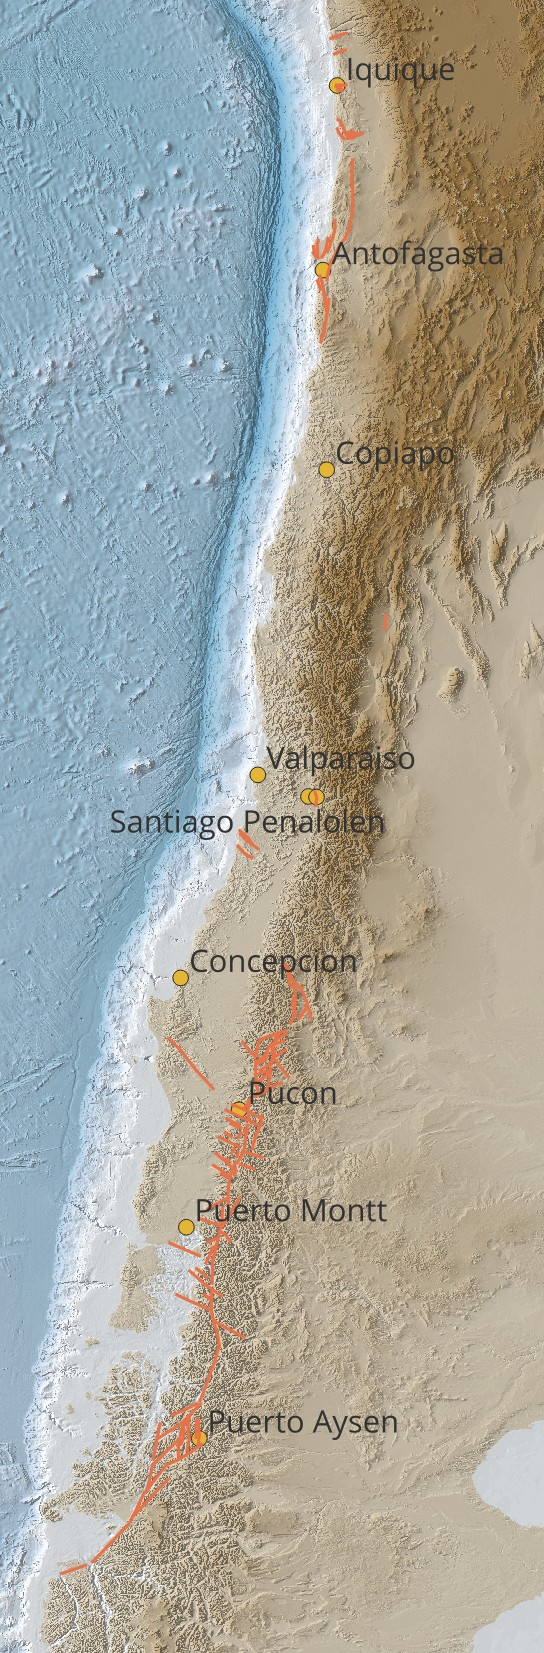
\includegraphics[width=0.4\textwidth]{../figures/cities}
	\end{figure}
		\end{columns}

\end{frame}
	\begin{frame}[t]
	\frametitle{Model Comparison - Hazard Curves}

		\begin{columns}
		\column{.6\textwidth}
			\begin{figure}
		\vspace{0.3cm}
		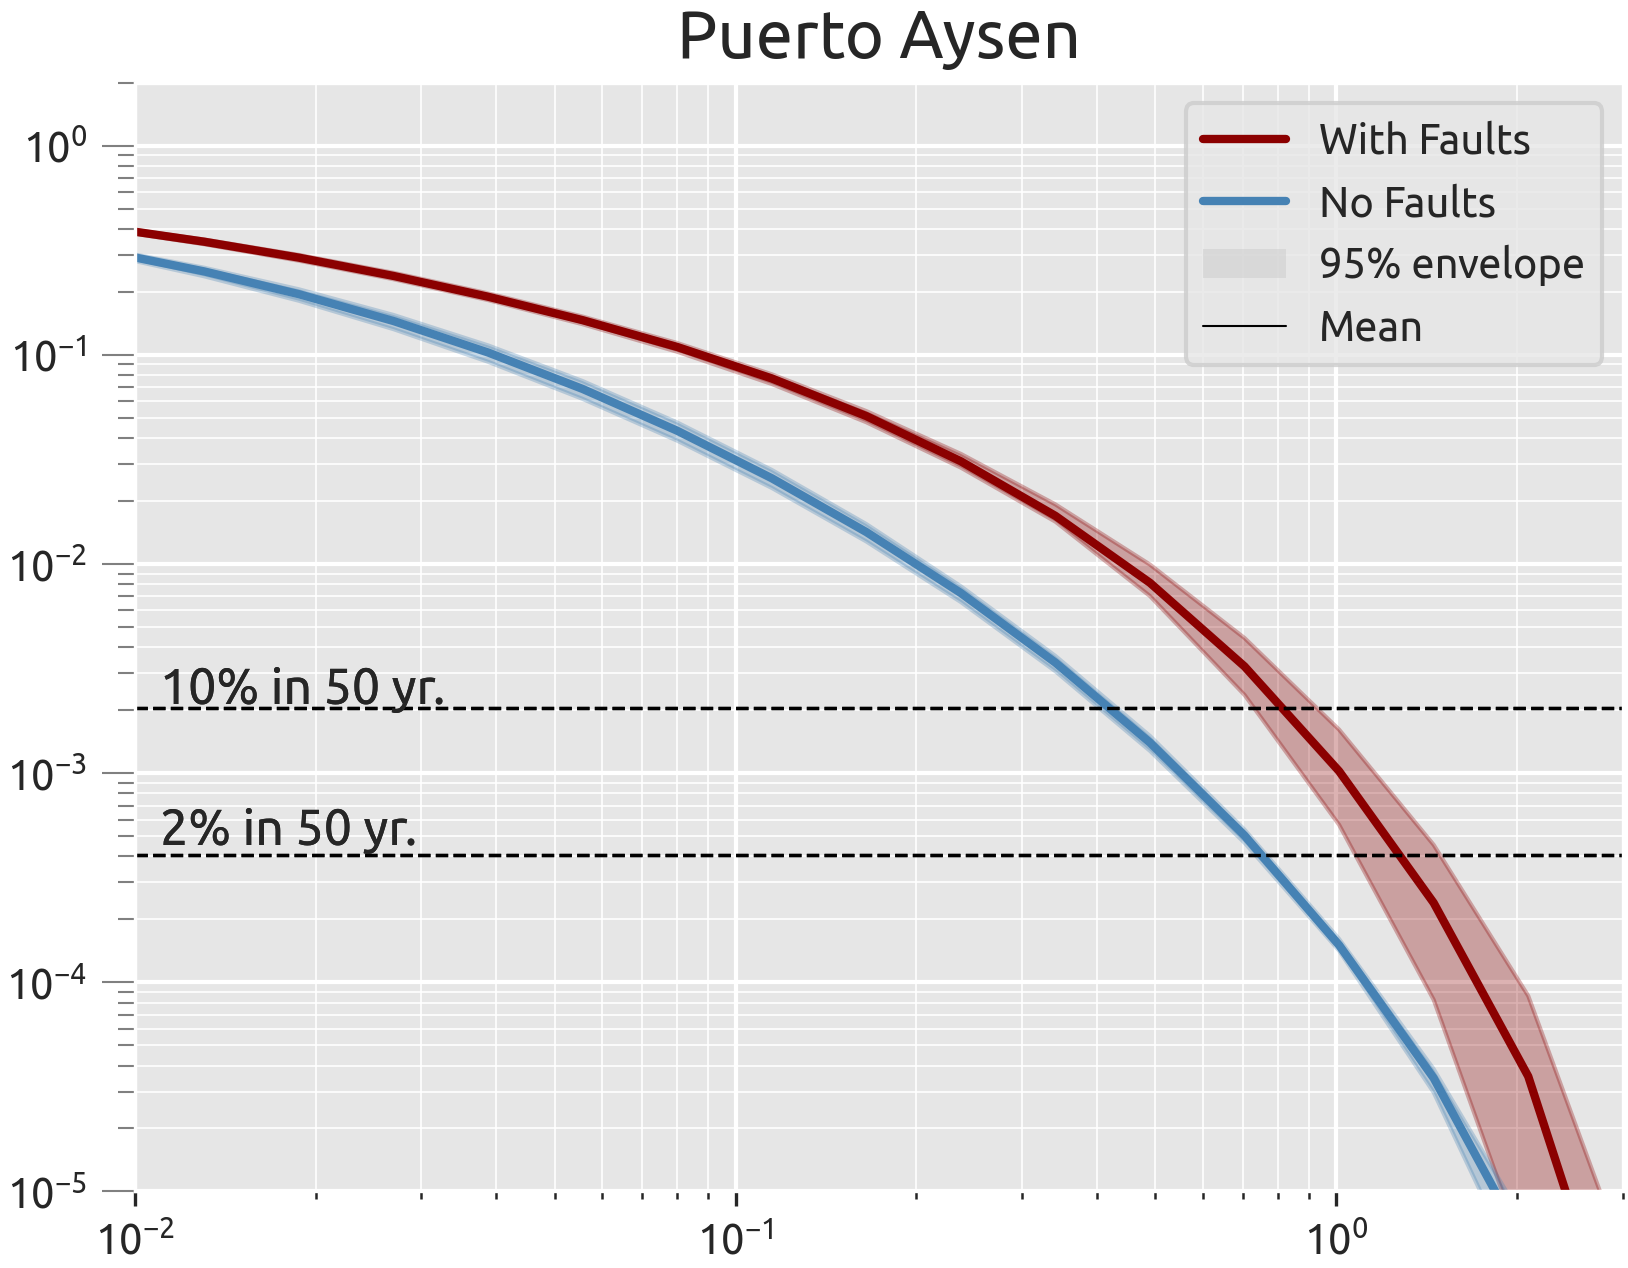
\includegraphics[width=0.8\textwidth]{../figures/Puerto Aysen}
	\end{figure}
		\column{.4\textwidth}
		\vspace{-1cm}
			\begin{figure}
		\vspace{0.3cm}
		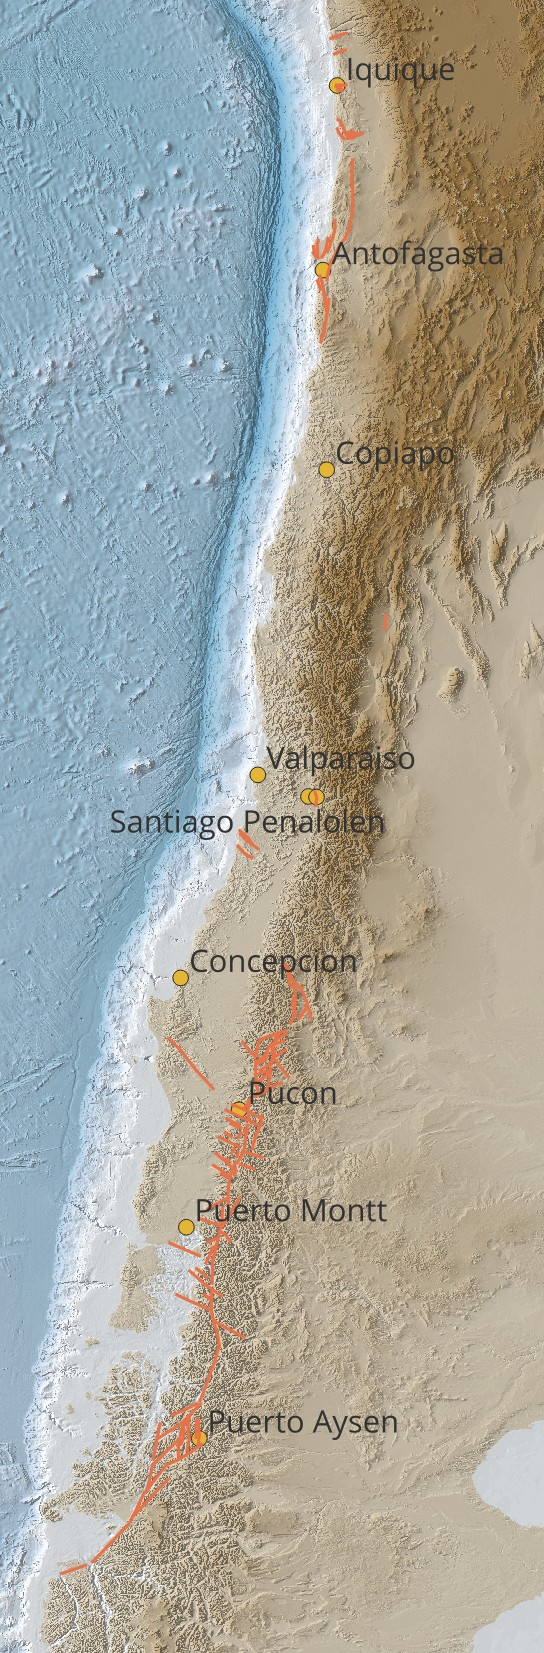
\includegraphics[width=0.4\textwidth]{../figures/cities}
	\end{figure}
		\end{columns}

\end{frame}

	\begin{frame}[t]
	\frametitle{Model Comparison - Hazard Curves}

	Absolute difference between model with and without faults. PGA at 10\% probability of exceedance in 50 years.
	\begin{figure}
		\vspace{0.3cm}
		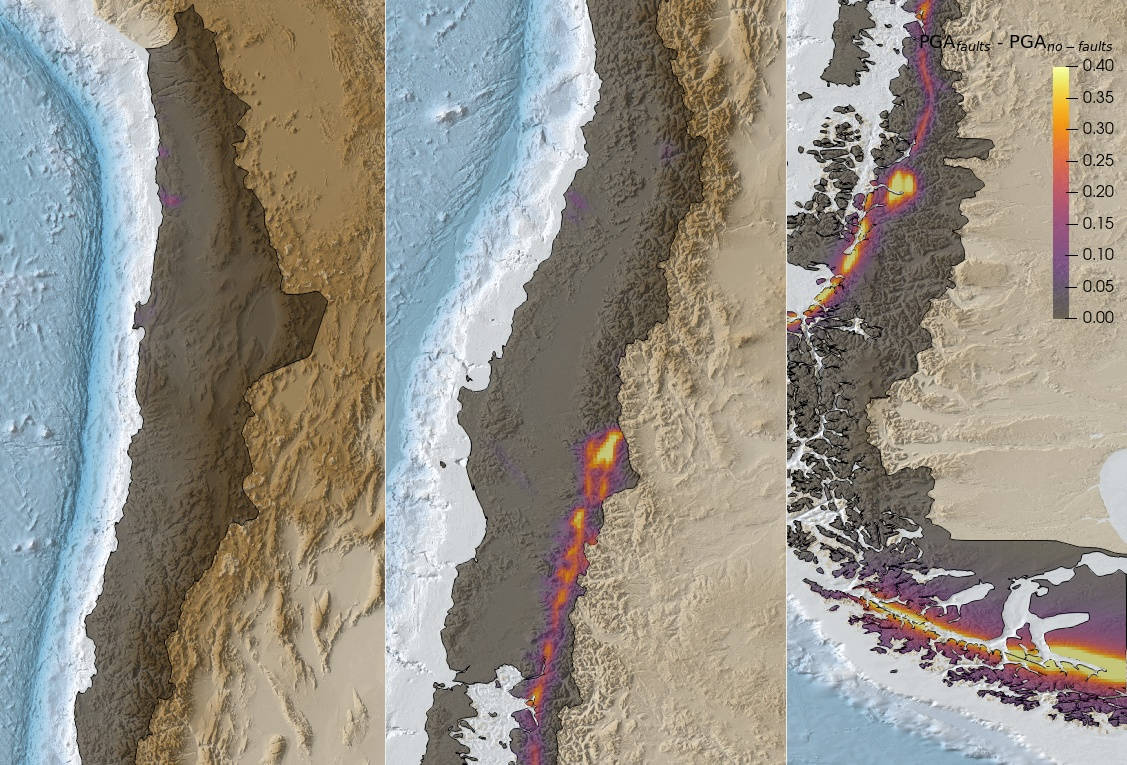
\includegraphics[width=0.6\textwidth]{../figures/abs_diff}
	\end{figure}
\end{frame}
	\begin{frame}[t]
	\frametitle{Model Comparison - Hazard Curves}

	Relative difference between model with and without faults. PGA at 10\% probability of exceedance in 50 years.
	\begin{figure}
		\vspace{0.3cm}
		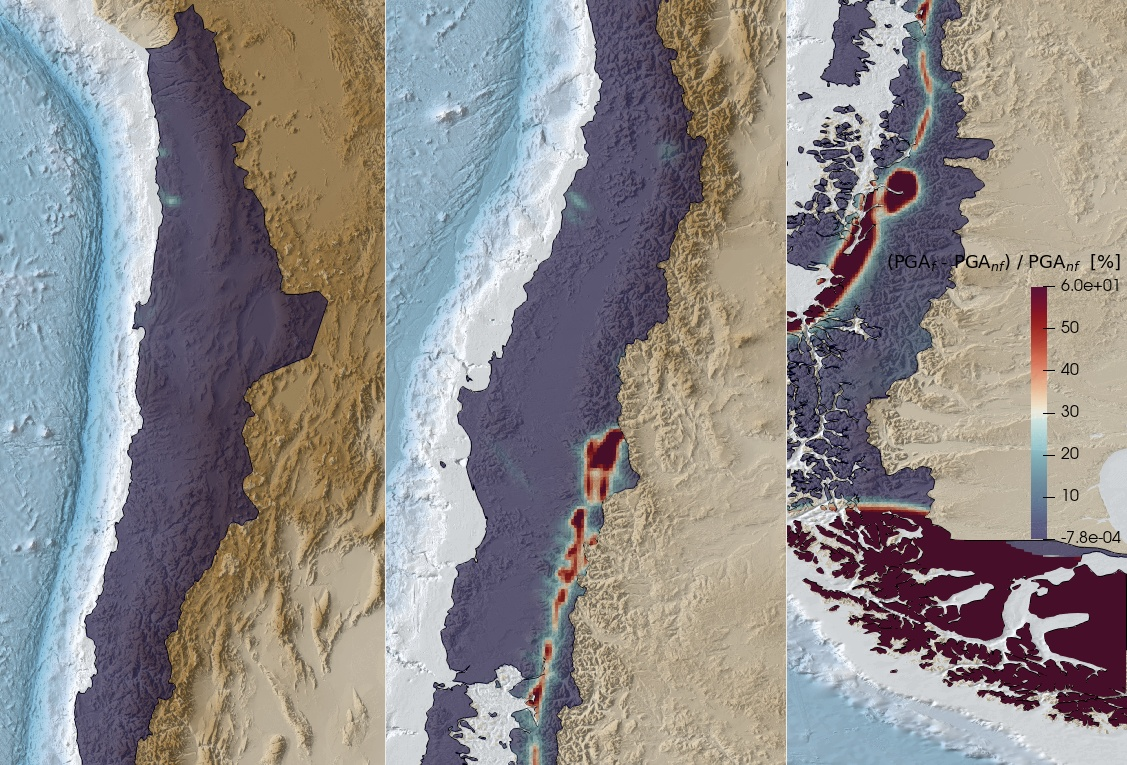
\includegraphics[width=0.6\textwidth]{../figures/rel_diff}
	\end{figure}
\end{frame}

	\end{document}